% !TEX root = main.tex

% \documentclass[12pt,a4paper]{article}
% \documentclass[acmlarge, manuscript,review,anonymous]{acmart}
\documentclass[acmlarge, manuscript,review]{acmart}

% \documentclass[sigchi]{acmart}

% Rights management information.  This information is sent to you
% when you complete the rights form.  These commands have SAMPLE
% values in them; it is your responsibility as an author to replace
% the commands and values with those provided to you when you

% complete the rights form.\
\copyrightyear{2024}
\acmYear{2024}
\acmConference[CHI '24]{Proceedings of the CHI Conference on Human Factors in Computing Systems}{May 11--16, 2024}{Honolulu, HI, USA}
\acmBooktitle{Proceedings of the CHI Conference on Human Factors in Computing Systems (CHI '24), May 11--16, 2024, Honolulu, HI, USA}
\acmDOI{XXXXXXXXXXXX}
\acmISBN{XXXXXXXXXXXX}
\usepackage[utf8]{inputenc}
\usepackage[english]{babel}
\usepackage{amsmath}
\let\Bbbk\relax
\usepackage{amssymb}
\usepackage{amsfonts}
\usepackage{graphicx}
\usepackage[all]{foreign}
\usepackage{cleveref}
\usepackage{booktabs}
\usepackage{colortbl}
\usepackage{tikz}
% \usepackage[left=3cm,right=2cm,top=2cm,bottom=2cm]{geometry}

%%%%%%%%%%%%%%%%%%%%%
\usepackage{here}
\usepackage{xspace}
\usepackage{textgreek}
\usepackage[section]{placeins}
\usepackage{subcaption}
% \title{Pointing Models for Users Operating Under Different Speed Accuracy Strategies}
\title{Pointing Beyond Fitts: Strategy, Movement Time Distributions, Local-Global Tradeoffs, and Generative Models}
\author{Julien Gori}
\email{julien.gori@sorbonne-universite.fr}
\orcid{0000-0002-3272-9176}
\affiliation{%
  \institution{Sorbonne Université, CNRS, Inserm, Institut des Systèmes Intelligents et de Robotique, ISIR}
  \city{F-75005 Paris}
  \country{France}
}

%%%%%%%%%%%%%%%%%%%%%%%%%%%%%% Custom commands
\newcommand{\mmt}{\ensuremath{\overline{\mt}}\xspace}
\newcommand{\mt}{\ensuremath{{\text{MT}}}\xspace}
\newcommand{\ide}{\ensuremath{{\text{ID}_e}}\xspace}
\newcommand{\D}{\ensuremath{{\text{D}}}\xspace}
\newcommand{\W}{\ensuremath{{\text{W}}}\xspace}
\newcommand{\strat}{\,\text{strat}\xspace}



\DeclareMathOperator*{\SumInt}{%
\mathchoice%
  {\ooalign{$\displaystyle\sum$\cr\hidewidth$\displaystyle\int$\hidewidth\cr}}
  {\ooalign{\raisebox{.14\height}{\scalebox{.7}{$\textstyle\sum$}}\cr\hidewidth$\textstyle\int$\hidewidth\cr}}
  {\ooalign{\raisebox{.2\height}{\scalebox{.6}{$\scriptstyle\sum$}}\cr$\scriptstyle\int$\cr}}
  {\ooalign{\raisebox{.2\height}{\scalebox{.6}{$\scriptstyle\sum$}}\cr$\scriptstyle\int$\cr}}
}

\begin{document}


\begin{abstract}
Traditional Fitts' law captures average trends in pointing tasks but ignores variability, strategy effects, and complex dependencies between movement time (MT) and effective index of difficulty (\ide). 
In this work, we adopt a probabilistic perspective to model the full distribution of MTs and \ide, and how this relationship depends on user strategy.
We analyze data from four empirical studies using three different experimental protocols that manipulate task constraints and user strategy across different input modalities, examining how speed and accuracy are traded off locally (within conditions) and globally (across conditions). We find strong global dependencies but minimal local dependencies, suggesting movements within a condition are largely functionally equivalent.
To capture behavioral distributions, we introduce a probabilistic \ide model, a bivariate Gaussian model linking \ide and mean movement time with strategy, as well as three models based on copulas and Exponentially Modified Gaussian (EMG) noise distributions that express the complete joint (\ide, MT) distribution, all of which are parametrized by user strategy. These three models are compared on their ability to faithfully reproduce summary statistics of the pointing datasets. This work offers a richer, distribution-and-strategy-based perspective on pointing performance. Code and parameters are provided for reproducibility and future research.
\end{abstract}
\maketitle

% position against other models
% copula section in appendix?
% motivation not clear
% protcols in appendix?
% where is the gap?


\section{Introduction\label{sec:introduction}}
Pointing tasks, such as selecting an icon with a mouse, are among the most fundamental interactions in human-computer interaction (HCI) \cite{card1978,soukoreff2004}. 
The dominant quantitative model of pointing, Fitts' law \cite{fitts1954,soukoreff2004,gori2018tochi}, predicts the mean movement time (MT) required to reach a target of width \(W\) at distance \(D\):
\begin{align}
	\mt & = a + b \log_2 (1 + \tfrac{D}{W}), \label{eq:fitts} \\
	          & \equiv a + b\,\text{ID}.
\end{align}
Here, $\text{ID}=\log_2 (1+D/W)$ is the index of difficulty, and the parameters $a$ and $b$ are empirically estimated. 
Fitts' law captures the speed-accuracy trade-off (SAT) in motor control: smaller targets, which require more precision, take longer to acquire. 
It has been validated across devices, modalities, and populations, and remains a cornerstone of input evaluation and interface design \cite{card1978,soukoreff2004}.

Yet, Fitts' law provides only a partial account of the SAT. It predicts average performance but ignores trial-to-trial variability. In reality, MTs are not fixed values but they are spread across a distribution, and some attempts are unexpectedly fast and precise while others are slow and inaccurate. 



Fitts' law also leaves no room for user strategy, where participants may favor speed or accuracy depending on instructions or personal preference \cite{zhai2004nominal,guiard2015}, which conflates intentional and unintentional variability, and as we will show, variability in MT and user strategy strongly influence observed responses: ignoring them oversimplifies pointing behavior and limits the predictive power of models.
To address these limitations, we adopt a \textit{probabilistic} perspective that treats both movement time and accuracy as random variables drawn from a joint distribution, conditioned on task and strategy.
Rather than assuming that going faster always means being less accurate, or that smaller targets always lead to lower MTs, we examine how user strategies and task properties influence the relationship between the observed MTs and accuracy.


We examine the dependence between movement time and accuracy at two levels of analysis.  At the \emph{local} level, we study the relationship between MT and accuracy within individual task conditions (given $D$, $W$, and strategy). 
At the \emph{global} level, we pool data across conditions. 
This distinction is important, as we find that the SAT is often weak or absent when examined locally, but emerges clearly at the global level. 
Understanding this contrast helps explain when trade-offs appear in experimental data and how they should be modeled.


To model this dependence, we rely on the exponentially modified Gaussian (EMG) distribution, which is parametric model that was previously validated to model MT distributions~\cite{gori2019,gori2018these,li2024,zhao2022}, but without accounting for strategy. 
The EMG model describes MT conditional on accuracy with a linear mean and a quadratic variance, thus imposing a specific dependency structure. 
While the EMG model captures important aspects of the SAT, it imposes the form of dependence a priori.
Thus, to allow for more flexibility, we also consider models based on \emph{copulas}, which describe the joint distribution of MT and accuracy without assuming a fixed pattern of dependence. 
Together, these approaches let us compare descriptions of the SAT across experimental conditions.


To ground these perspectives, we analyze pointing data collected under three experimental protocols that differ in how accuracy is defined: 
(1) the classic \emph{Fitts} protocol, where accuracy is set by target width $W$; 
(2) a \emph{pure strategy} protocol, where accuracy is determined by participants in line with experimenter instructions; and 
(3) a combined \emph{Fitts-with-strategy} protocol that merges both task and strategy constraints. 
Together, these protocols reveal how task properties and strategy interact to shape pointing performance.

\paragraph{Contributions.} 
This paper makes the following contributions:
\begin{itemize}
	\item A theoretical analysis that shows why Pearson correlation is not adapted to evaluate the fitness of models that predict the joint distribution between MT and accuracy.
	\item New probabilistic models of pointing linking movement time to accuracy, building on EMG, copulas and a bivariate Gaussian model that capture the dependency between MT and accuracy in different ways. 
	\item Empirical findings across three protocols, that show that the SAT is often weak locally but emerges globally, and that strategy systematically shifts these patterns. 
	\item Open resources: reusable model parameters and code for generating realistic pointing data, supporting replication and extension by the HCI community. The code used for this paper is available at the following \href{https://github.com/jgori-ouistiti/pointing_models}{\color{blue} repository}.
\end{itemize}

By moving beyond deterministic, strategy-agnostic models that describe average movement times, this work provides a richer account of the SAT in pointing and introduces tools that better reflect the variability and strategies observed in real interaction.




% in this work we emphasize characterizing the statistical dependence between speed and accuracy. Additionally, when participants prioritize accuracy, there is on average an increase in pointing time, which leads to a wider pointing time distribution~\cite{gori2018these, gori2019, li2024, zhao2022}\footnote{Similar results have also been demonstrated for reaction time distributions~\cite{wagenmakers2007}.}. Understanding precisely how this spread increases is central to our analysis. To model the pointing data, among other better-known techniques, in this work we leverage copulas, which are statistical functions that entirely and uniquely capture the dependency structure between variables which to our knowledge have never been used in HCI before.





% This ensures the model can be widely applicable \eg used in simulation studies, see \autoref{subs:mmt::distrib}.
	
	
% \eg as a low-level control module as in~\cite{jokinen2021,langerak2022}, and overall, will be more widely applicable and more explanatory (while likely somewhat sacrificing precision).



% Since Fitts' seminal 1954 work~\cite{fitts1954}, and its introduction by Card and colleagues in HCI in 1978~\cite{card1978}, movement modeling has greatly advanced.
% While Fitts' law only describes \emph{endpoints}, motor control models now propose description of entire \emph{trajectories} produced during pointing tasks~\cite{todorov2002, saveriano2023, fischer2021, gori2020, gori2023}.
% While Fitts' law only describes \emph{means} of movement times, several models now describe \emph{distribution} of movement times, usually using asymmetric distributions~\cite{chapuis2007, jude2016, gori2019,li2024,zhao2022, nieuwenhuizen2016}.



% One aspect that has been less studied in models of pointing is its strategic aspect. Most people will regularly over or under utilize the target width W~\cite{soukoreff2004}, creating, according to Zhai and colleagues, \textit{an additional subjective layer of SAT}~\cite{zhai2004nominal}, which the current formulations of Fitts' law do not capture \textit{a priori}. But models that describe how users point under different speed-accuracy strategies (hereafter simply strategies) are essential when addressing users with varying incentives.
% For example, people will favor accuracy in contexts where safety matters critically~\cite{guiard2011b}.



% One exception is the Weighted Homographic (WHo) model of Guiard and Rioul~\cite{guiard2015} described \autoref{subsub:who}, which relates movement time, movement precision, strategy, and effort. The WHo model was recently used as a low level control module in hierarchical models of user behavior~\cite{jokinen2021, langerak2022}, where a high level controller learns to be more cautious in contexts where the cost to recover from errors is higher.
% However, the WHo model is not an appropriate tool to describe regular user behavior, since it was built as a model of \textit{ultimate} performance; it does not describe the entire distribution of data, but instead, it describes the limit speed and accuracy performances one can obtain(the \textit{front of performance}, in Guiard and Rioul's words, also see \autoref{subs:rw::twolaws}). In Guiard and Rioul's work, the WHo model is fitted only on the best 10 measures, out of 400! Works that use the WHo model thus use an overly optimistic model of user behavior.
% Another relevant work is due to Zhai~\etal~\cite{zhai2004nominal}, who, moving away from the pure ``task-based'' perspective of Fitts' law, introduce an index of target utilization to quantify strategic effects on pointing, which is shown to be an important predictor for movement time.


% Following Guiard \etal{} and Zhai \etal{}, the goal of this work is to propose and compare candidate pointing models for users operating under different strategies. Our modeling objectives are as follows:
% \begin{itemize}
% 	\item The model should describe the entire distribution of movement times, and not just the means (as in Fitts' law) or extrema (as in WHo, also see~\cite{gori2017two, gori2019, li2024}). This ensures the model will be widely applicable \eg used in simulation studies, see \autoref{subs:mmt::distrib}. This implies MT should be interpreted in this work as a random variable, whose distribution we characterize.
% 	\item The model should be parametric, so that it can be easily interpreted, and its parameters easily identified. The distributions we model in this work could alternatively be learned by machine learning techniques using so-called generative models see \eg~\cite{harshvardhan2020} for a review on the topic.  Compared with the machine learning approach, we believe that ours, being explicit and parametric, will facilitate the model being re-used and adapted by others \eg as a low-level control module as in~\cite{jokinen2021,langerak2022}, and overall, will be more widely applicable and more explanatory (while likely somewhat sacrificing precision).
% 	\item One of the parameters of the model should map directly to the concept of strategy \ie a bias towards speed or accuracy when producing movements, to fill the gap identified beforehand.
% \end{itemize}



% \paragraph{Notations} $\mathcal{N} (\mu, \Sigma)$ refers to the (multivariate) Gaussian distribution with mean $\mu$ and covariance matrix $\Sigma$, $\mathcal{E}(\lambda)$ refers to the exponential distribution with mean $\lambda$, $\mathbb{E}[X]$ refers to the mathematical expectation (population mean) of $X$, $\text{Var}(X) = \mathbb{E}[(X - \mathbb{E}[X])^2]$ refers to the (population) variance of $X$. We use $X \sim \mathcal{D}$ to indicate that the random variable $X$ is distributed following the distribution $\mathcal{D}$.
% We use R-style formulas to describe statistical models for example, $A \sim X*Y + (1|Z)$ is a linear mixed effect model with random intercepts for groups of $Z$, with main effects $X$ and $Y$, and with an interaction effect between $X$ and $Y$.

\section{Related work\label{sec:rw}}
Pointing is an instance of a goal-directed movement, which has been extensively described in the motor control literature (see \eg~\cite[Section 2]{todorov1998} or \cite{elliott2017} for an introduction). The SAT in pointing has been known at least since Woordworth~\cite{woodworth1899}, and is classically captured by Fitts' law for goal directed movements, and Schmidt's law~\cite{schmidt1979} for fast, open loop movements.
In HCI, pointing is one of the fundamental elementary interactions of users with GUI; the topic has, and continues to attract attention.


\subsection{Fitts' law extensions}
Many studies have extended Fitts' law, and namely its applicability to novel paradigms such as 2D and 3D pointing, by proposing a novel index of difficulty.
For instance, Accot and Zhai~\cite{accot2003} review several indices for bivariate pointing, with additional insights provided by~\cite{grossman2005b}, while Murata and Iwase~\cite{murata2001} extend the framework to trivariate pointing. 
These models however do not provide MT distributions and overlook the impact of user strategy on performance. 
Another line of research focuses on modeling the spatial distribution of movement endpoints. Notable examples include the \textit{sum-of-Gaussians} models~\cite{bi2013, yamanaka2020, zhang2023}. While these models capture endpoint distributions, their treatment of movement time remains based on averages. Additionally, no sum-of-Gaussians model incorporates parameters that directly account for user strategy to our knowledge.


% Grossman and Balakrishnan~\cite{grossman2005b} defined an ID in terms of the probability of hitting the target a concept that may initially seem tied to user strategy. However, as the authors clarify, this probability is influenced by geometric factors, specifically the likelihood of hitting the target in a ballistic, open-loop movement, but as noted by Gori \etal~\cite{gori2020}, strategy differences are more pronounced during the corrective phase of movement\footnote{This phase, crucial for precise tasks, can last up to four times longer than the initial ballistic phase, see \cite{gori2020}.}.


\subsection{Pointing with different strategies}
Most people will regularly over or under utilize the target width W~\cite{soukoreff2004}, creating, according to \citeauthor{zhai2004nominal} an additional subjective layer of speed-accuracy tradeoff~\cite{zhai2004nominal}. This strategic choice may be affected by context, for example people will favor accuracy in when safety matters critically~\cite{guiard2011b}.
Various works have thus investigated the effect of strategy on pointing performance. This includes work on the invariance of throughput for different user strategies~\cite{mackenzie2008,olafsdottir2012,batmaz2022} and the comparison of evaluations of different interaction techniques~\cite{yamanaka2023}, but has also lead researchers to define variations on Fitts' protocols, further described \autoref{subs:background::protocols}. Here we focus on existing models that account explicitly for strategy.
\subsubsection{The effective index of difficulty \ide}
Because participants do not always follow the accuracy constraint as enforced by W, Crossman~\cite{crossman1957} suggested a correction that was popularized in HCI by Mackenzie~\cite{soukoreff2004, gori2018tochi}, called the effective index of difficulty\footnote{The index generalizes to multiple dimensions, but not without controversies, see \eg~\cite{wobbrock2011,mackenzie1992,gori2023}.}
\ide, which is a function of the actual measured standard deviation of endpoints $\sigma$
\begin{align}
	\mt & = a + b\,\log_2 \left(1 + \frac{D}{4.133\sigma}\right)                       \equiv a + b \log_2 \left(1 + \frac{D}{W_e}\right)= a + b\,\text{ID}_e        . \label{eq:ide}
\end{align}
ID$_e$, as a function of $\sigma$, is a direct measure of accuracy, and may only be computed a posteriori on observed data.

\subsubsection{The index of target utilization\label{subs:background::target_util}}
Zhai~\etal~\cite{zhai2004nominal} investigated the effect of strategy on pointing by introducing an index of target utilization
\begin{align}
	I_U = \log \frac{W_e}{W}.
\end{align}
$I_u$ measures the effect of strategy, because, as shown in \cite[Appendix 3]{gori2018tochi}, when the spatial distribution of endpoints is Gaussian\footnote{which is a reasonable assumption that holds well in practice~\cite{soukoreff2004, gori2020}} $W_e = \frac{2.066}{\sqrt{2}\text{erf}^{-1}(1-\varepsilon)} W$, where $\varepsilon$ is the rate at which participants miss the target. Thus, $I_u$ is a non-linear transformation of the miss rate $\varepsilon$. 
The key finding from \citeauthor{zhai2004nominal}~\cite{zhai2004nominal} for our purposes is that the post-hoc correction $W_e$ of \autoref{eq:ide} does not fully eliminate the influence of participant strategy: even when using \ide, the parameters of Fitts' law vary with strategic choices. Moreover, they showed that D and W have effects on movement time beyond their ratio D/W. These results imply that \ide should not be treated as a pure one-dimensional proxy for task difficulty, but rather as a quantity shaped jointly by ID, D, W, and participant strategy. This observation motivates our modeling of its distribution, see \autoref{sec:outline}.



\subsubsection{The WHo model\label{subsub:who}}
To our knowledge, \citeauthor{guiard2015}'s WHo model~\cite{guiard2015}, which follows from the ressource allocation model described~\cite{guiard2011b}, is the only parametric model that describes pointing data with an explicit parameter for strategy.
% Guiard and Rioul~\cite{guiard2015} listed 6 axioms that any \textit{deterministic} theory of the SAT should respect
% \begin{enumerate}
% 	\item[axiom 1] Each participant has a minimum average movement time $x_0$ that they can reach
% 	\item[axiom 2] With relative precision $y = \sigma/D$ with $\sigma$ the standard deviation of endpoints, each participant has a minimum relative precision $y_0$ that they can reach.
% 	\item[axiom 3] The function $f$ that links x to $y$, $y=f(x)$ is decreasing and convex
% 	\item[axiom 4] For a given participant effort $k$, there is an operation such that $x \odot y = k$
% 	\item[axiom 5] Effort invested is never total: participants may routinely perform worse than ideally possible.
% 	\item[axiom 6] Participants can modulate how they allocate resources to speed versus accuracy. 
% \end{enumerate}
% The WHo model
% \begin{align}
% 	(y-y_0)^{1-\alpha} (x-x_0)^{\alpha} = k
% \end{align}
% satisfies axioms 1--4, and is fit on the convex hull of the scatterplot in the ($x$, $y$) space to satisfy axiom 5. A $\beta \in [0,1]$ parameter for strategy (axiom 6) is defined as
% \begin{align}
% 	\beta = \frac{\lambda}{1 + \lambda}\text{, with } \lambda = -\frac{dy}{dx}.
% \end{align} 
However, the WHo model does not describe a distribution of movement times. Instead it characterizes the ``best average'' samples, %(axioms 1, 2 and 5), 
which is operationalized by fitting not on all data points but only on the convex hull of block averages: In their work, the WHo model is fit on only 10 block averages out of 400, but \citeauthor{guiard2015} never described what the distribution of movement times could look like within their WHo model.

\subsection{Pointing models that describe the distribution of MT}
\subsubsection{Fitts' law, regression, and the implicit noise model \label{subs:rw::fitts}}
The expression for Fitts' law \autoref{eq:ide} masks an underlying statistical model that assumes additive, centered noise\footnote{Because most researchers applying Fitts' law rely on ordinary least squares (OLS), they also implicitly assume the noise is uncorrelated and homoscedastic (has equal variance), as OLS is only optimal under these conditions.}:
\begin{align} \mt = a + b\ide + \text{noise (additive)}, \quad \mathbb{E}[\text{noise}] = 0 \text{ (centered)}. \label{eq:mt} \end{align}
Pearson's $r$ is commonly used as a goodness-of-fit measure. % because for linear models with OLS $r^2 = R^2$, where $R^2$ is the so-called coefficient of determination which reflects the proportion of variance in the dependent variable that is explained by the model while simultaneously assessing the model’s linearity~\cite{lee1988}. 
However, as shown by Drewes~\cite{drewes2013} and Gori~\etal~\cite{gori2018chi}, the Pearson correlation between MT and \ide, $r(\mt, \ide)$, often yields moderate to low values in practice on pointing datasets, with some cases showing correlations close to zero~\cite{gori2018tochi}.

In fact, to mitigate variability in MT and increase the goodness-of-fit measure, researchers typically compute the sample average of MT, denoted in the remainder of the work as \mmt\footnote{See~\cite{gori2017two} for further discussion on considering the sample average.}, before calculating $r$. Consequently, the model actually considered by many researchers is:
\begin{align}
	\mmt = a + b\ide + \text{noise (additive)}, \quad \mathbb{E}[\text{noise}] = 0 \text{ (centered)}, \label{eq:mmt}
\end{align}
with the goodness-of-fit measure being $r(\mmt, \ide)$. Fitts' law is thus essentially a Gaussian model for average pointing time \mmt.


\subsubsection{Asymmetric MT distributions and the Exponentially Modified Gaussian (EMG) noise model \label{subs:rw::emg}}
Rather than averaging out the noise as in \autoref{eq:mmt} and describing only \mmt, other works model the entire noise distribution instead, and show that the conditional distribution of MT for a given ID or \ide level is distributed according to an asymmetric, positive (right) skewed~\cite{gori2018these,gori2019,zhao2022, jude2016,nieuwenhuizen2016, li2024,chapuis2007} distribution.
While several distributions have been suggested, including gamma, Gumbel and lognormal, we follow Gori and colleagues~\cite{gori2018these,gori2019, li2024}, and Zhao \etal~\cite{zhao2022} who considered an Exponentially Modified Gaussian (EMG) noise model: it is positive, is assymetric, %(except when $1/\lambda << \sigma^2$)
has parameters that are easy to interpret and has shown good performance, including when modeling steering data~\cite{wang2021}.%, and there exist tools to aid in its parameter estimation~\cite{li2024}.



% The EMG model for movement time defines MT as the sum of a Gaussian ($G$) and an Exponential ($E$) random variable~\cite{gori2019, li2024} 
% \begin{align}
% 	& \mt   = G + E, \label{eq:emg}                                                                 \\
% 	& G           \sim \mathcal{N}(\beta \mathbf{x}, s) = a + b\,\ide + \mathcal{N}(0,s), \text{ with }\beta = [a,b] \text{ and } \mathbf{x}  = [1, \ide]^t \label{eq:emg1} \\
% 	& E       \sim \mathcal{E}(\lambda)
% \end{align}
% The $G$ part models pointing as the standard Fitts' law with Gaussian noise, in line with \autoref{eq:mt}, as reflected by the right hand side of \autoref{eq:emg1}. $E$, being an exponential random variable, is always positive  meaning that the EMG model only allows deviations from Fitts' model that increase movement times. This idea was justified for example in~\cite{gori2017,gori2018chi, gori2018these} and builds on arguments of the WHo model\autoref{subsub:who}. That the positive random variable is exponential can be justified by a maximum entropy~\cite{jaynes1957} argument, see~\cite{gori2019}.


Gori~\cite{gori2018these} further showed that a \textit{quadratic variance} model, where the standard deviation of the MT distribution increases linearly with its mean, provided a good fit to empirical data,
% \begin{align}
% 	E \sim \mathcal{E}(\lambda \mathbf{x}), ~\lambda = [\lambda_0, \lambda_1] \label{eq:emg2},                                 
% \end{align}
which was later confirmed by \citeauthor{zhao2022}~\cite{zhao2022} who similarly found that quadratic variance models provided the best fit among the models they tested.


The probability density function of the EMG model with linear increasing standard deviation reads
\begin{align}
	f_{\mt}(mt) = \frac{1}{2\lambda\mathbf{x}} \exp\left(\frac{1}{2\lambda\mathbf{x}}(2\beta\mathbf{x} + \frac{s^2}{\lambda\mathbf{x}} - 2mt)\right) \mathrm{erfc}\left(\frac{\beta\mathbf{x} + \frac{s^2}{\lambda\mathbf{x}} - mt}{\sqrt{2} s}\right),
\end{align}
where erfc is the complimentary error function, $\mathbf{x} = \left[1, \ide \right]^T$, $\lambda = \left[ \lambda_0, \lambda_1 \right]$ and $\beta = \left[ a, b\right]$. Although this density is analytically quite complex, it has a simple conditional mean, where \mmt increases linearly with \ide
\begin{align}
	\mathbb{E}[\mt|\ide] = \beta \mathbf{x} + \lambda \mathbf{x} = a + \lambda_0 + (b + \lambda_1) \ide, \label{eq:emg_mean}
\end{align}
and a quadratic conditional variance, where the variance of MT increases quadratically with \ide
\begin{align}
	\text{Var}(\mt|\ide) = s^2 + (\lambda \mathbf{x})^2 = s^2 + \lambda_0^2 + 2\lambda_0\lambda_1\ide + \lambda_1^2\ide^2. \label{eq:emg_conditional_variance}
\end{align}
Throughout this work, we fitted the EMG distributions when needed with maximum likelihood estimation. 





% One sees the EMG distribution results from adding an exponential noise term \autoref{eq:emg2} to a more classical centered Gaussian noise model \autoref{eq:emg1}.
% Depending on the parameter values, the EMG distribution can behave like a Gaussian ($s >> \lambda \mathbf{x}$), like an exponential ($s << \lambda \mathbf{x}$) or in between~\cite{gori2019}.


\subsection{Models that simulate entire trajectories\label{rw:simulators}}
\subsubsection{Optimal feedback control models}
Several optimal feedback control (OFC) models for pointing have been applied in HCI~\cite{klar2023,fischer2022}, following from the seminal work by Todorov and Jordan~\cite{todorov2002}. These predict complete movement trajectories as well as their spatial variability.
Unfortunately, these models are not well suited to predict movement time and its associated variability, since OFC doesn't have an intrinsic mechanism to stop controlling, and thus it requires defining a stoping condition (see \eg \cite[Section 3.4]{qian2013}). \footnote{There are two possibilities: either a fixed horizon is used, which requires specifying in advance the movement duration, or an infinite or receding horizon is used. In that case, movements are perpetual, except if a stopping condition (usually arbitrary) is formulated.}
Solutions to this problem include integrating an explicit cost for time, as in~\cite{berret2016}, but to our knowledge there is currently no OFC model that has predicted realistic MT distributions.
Reinforcement learning approaches, which can be viewed as methods to solve optimal control problems when the dynamics of the controled system are unknown, share the same limitation: although they can learn policies that lead to realistic movement trajectories and can produce data compatible with Fitts' law~\cite{ikkala2022, charaja2024}, they similarly require stopping criteria or cost of time~\cite{fischer2022}, and to our knowledge, have never been shown to generate realistic distributions of movement times.


\subsubsection{Simulation models}
Optimal control models typically have closed-form solutions or can be computed numerically with sufficient speed to enable real-time implementation. In contrast, more complex approaches, to which we refer as simulation models, have also been proposed. For instance, Do et al.~\cite{do2021} present an intermittent control model for pointing that incorporates various sources of variability, including motor and perceptual noise. However, this model does not report movement time (MT) variability, and the role of user strategy in its framework remains unclear. Additionally, the model required six days of training.
Similarly, Moon et al.~\cite{moon2024} introduce a movement model trained using proximal policy optimization, a deep reinforcement learning technique, but the study does not report on MT variability and required approximately 40 hours of training.
Thus, while simulation models can be used to generate movement time trial data, to our knowledge, no such results have been reported, nor on the variability of MT. Moreover, while it should be possible, it remains unclear at this point how these models could be adapted to account for user strategy. Finally, their lengthy training times and the efforts required for their implementation undermine their utility as simple, parametric models, which are the focus of this work.





\section{Preliminaries}

\subsection{Theoretical analysis of the $r^2(\mmt, \ide)$ correlation \label{subs:theory_rsq}}


The goodness of fit of Fitts' law is usually justified via Pearson correlation $r^2(\mmt, \ide)$, which is close to 1 in many experiments where accuracy is manipulated by W~\cite{soukoreff2004}.
However, we show that many different MT distributions can achieve $r^2(\mmt, \ide)$ close to 1. Thus, using alignement with Fitts' law is a weak criterion to assess the fit of a model for distribution of movement times.

\begin{proposition}\label{prop}
	Any conditional distribution $p(\mt|\ide)$ will reach $r^2(\mmt, \ide) = 1$ if it has a conditional expectation $\mathbb{E}[\mt|\ide]$ that is linear in \ide.
\end{proposition}

The proof is given in \autoref{app:proofs}, and relies on the fact that Pearson correlation is a function of the covariance, which measures linear deviations from the mean. Several distributions that have been previously used for modeling pointing times satisfy this condition
\begin{itemize}
	\item The EMG model with quadratic variance~\cite{gori2018these,gori2019, li2024,zhao2022} (\autoref{eq:emg_mean}) has linear conditional mean.
	\item A gamma~\cite{jude2016} distribution with shape $k$ and scale $\theta$ has mean value $k\theta$. Having $k$ or $\theta$ increase linearly with \ide would fulfill the condition.
	\item A generalized extreme value~\cite{chapuis2007} distribution GEV$(\mu, \sigma, s)$ has a mean value that increases linearly with $\mu$. Having $\mu$ as a linear function of \ide would thus also fulfil the condition.
\end{itemize}
There are many more distributions possible, since one can force a conditional linear mean into any continuous distribution whose mean can be set freely.
Two important takeaways follow: First, models of movement time must have a conditional mean linear in \ide to satisfy Fitts' law.
Second, it motivates the need to turn to measures of dependences that are more sophisticated than Pearson correlation.

In practice, \mmt may refer to different aggregated quantities, depending on how data are collapsed across conditions, participants, and repetitions~\cite{olafsdottir2012}. For example: (i) averaging across all (D,W) pairs~\cite{soukoreff2004}, (ii) averaging over ID levels (noting that multiple (D,W) pairs can map to the same ID~\cite{gori2018chi}), or (iii) aggregating across participants~\cite{accot1997,mackenzie2008}. When blocks are repeated, aggregation may again be performed over repetitions~\cite{jude2016,guiard2011}. Each additional aggregation step tends to inflate 
$r^2(\mmt,\ide)$ by the same mechanism outlined in the proof of the Proposition.


\subsection{Measuring the dependence between two random variables with bivariate copulas\label{sec:copula}}

% \subsubsection{Measures of association}
% Measures of association~\cite{nelsen2006} quantify the strength and direction of the relationship between two variables; they are (in most cases) weaker than measures of dependence in the sense that independence implies an absence of association, but the converse is not true\footnote{``Correlation does not imply causation''}.

% \paragraph{Pearson's $r$} Pearson's $r$ is a well-known measure of association that captures the \textit{linear relationship} between two random variables. A value of $1$ (resp. $-1$) means that the data from the two variables are perfectly aligned with a positive (resp. negative) slope. One well-known weakness of Pearson correlation is that a null value only indicates the absence of a linear association, even though non-linear associations are common, see for example Anscombe's quartet~\cite{anscombe1973}.

% \paragraph{Rank correlations: Spearman's $\rho$ and Kendall's $\tau$}
% Spearman's $\rho$ between two variables equals Pearson's $r$ between the \textit{ranks} of the variables; as a result it allows capturing monotonic (increasing or decreasing, which includes linear but many more) relationships between variables. It will have a value of $1$ (resp. $-1$) when the order of the sorted values of one variable is the same (resp. opposite) as the other variable.
% Kendall's $\tau$ is a different rank correlation metric, which, for our purpose, has the same properties as $\rho$.\footnote{\dots{} but in general does not have the same value~\cite[Chapter 5]{nelsen2006}. It is more sensitive to smaller rank inversions or ties. Both $\rho$ and $\tau$ can be derived from the same general correlation coefficient~\cite{kendall1948}.}



% These measures of association (usually $\tau$) can sometimes be mapped to the copula's parameters $\theta$, for example for the Gumbel copula specified above $\tau = \frac{\theta -1}{\theta}$, meaning that the dependence between two variables can be steered by a few parameters only (in this case 1).
In the previous section, we argued that Pearson correlation $r^2$ is a limited tool for evaluating Fitts' law models because it only reflects linear associations between mean MT and ID$_e$, and ignores other aspects of the joint distribution. To move beyond this limitation, we need methods that capture dependence structures more generally.


Copulas are mathematical functions that describe the dependence structure between two random variables, independent of their individual distributions. Any bivariate joint distribution can be decomposed into its marginals, which describe the behavior of each variable separately, and a copula, which describes how the two variables are linked (Sklar's theorem~\cite{nelsen2006}). Thus copulas ``couple''~\cite[Chapter 1]{nelsen2006} two marginals, and capture the dependence between two variables even when the actual scales or distributions of the variables have been factored out, thus going well beyond what linear correlation can reveal.



To illustrate the usefulness of copulas, consider a model for generating synthetic human height and weight data. Both height and weight are likely to follow a Gaussian distribution, and with access to a basic anthropomorphic dataset, we can estimate their parameters. 
A simple, yet flawed, approach to generating realistic human data would be to treat height and weight as independent variables: first sampling height, then independently sampling weight. This approach, however, ignores the natural correlation between height and weight: taller individuals tend to weigh more than shorter individuals, and this relationship needs to be captured for a realistic model.
Copulas not only allow us to imply a dependence structure between weight and height; but different copulas specify different forms of dependencies between weight and height.


\autoref{fig:copulas_explained} illustrates how the Gaussian copula shapes a joint distribution: In (d), the two marginals (a) and (b) are independently combined. In (e), the two marginals are coupled with a Gaussian copula (c). For this illustration, we have used realistic marginal distributions for MT (a) and ID (b). Note that in both jointplots (d) and (e), the estimated marginals are identical, but notice how the datasets differ. In particular, we see that the dataset obtained with the Gaussian copula has variance that increases with ID levels, which is characteristic of pointing data~\cite{gori2018these}.



% \begin{figure}[htbp]
% 	\centering
% 	\begin{tikzpicture}
% 		\draw (0,0) node[name = 00]{\includegraphics[width=.3\textwidth]{img/copula_scheme_00.pdf}};
% 		\draw (0,0) ++ (6,0) node[name = 01]{\includegraphics[width=.3\textwidth]{img/copula_scheme_01.pdf}};
% 		\draw (01) ++ (6,0) node[name = copula]{\includegraphics[width=.4\textwidth]{img/copula_scheme_4.pdf}};
% 		\draw (2, -8) node[name=indep]{\includegraphics[width=.4\textwidth]{img/copula_scheme_3.pdf}};
% 		\draw (10, -8) node[name=cop]{\includegraphics[width=.4\textwidth]{img/copula_scheme_5.pdf}};
% 		\draw[-latex] (00.south) -- (indep.north);
% 		\draw[-latex] (01.south) -- (indep.north);

% 		\draw (cop.north) ++ (0,1.5) node[circle, draw=black, name = func]{\phantom{x}};
% 		\draw[-latex] (00.south) -- (func);
% 		\draw[-latex] (01.south) -- (func);
% 		\draw[-latex] (copula.south) -- (func);
% 		\draw[-latex] (func) -- (cop);

% 		\draw (00.north) node[above]{(a)};
% 		\draw (01.north) node[above]{(b)};
% 		\draw (copula.north) node[above]{(c)};
% 		\draw (indep.south) node[below]{(d)};
% 		\draw (cop.south) node[below]{(e)};

% 	\end{tikzpicture}
% 	\caption{How copulas couple two marginals. (a) represents the marginal distribution for MT, here an EMG model. (b) represents the marginal distribution for ID, here a Gaussian model. One can sample independently from MT and ID to obtain a joint (MT, ID) distribution as in (d), however, it does not reflect the fact that low ID movements have usually smaller durations. (c) is a Gaussian copula, which introduces a symmetric dependence between the variables. Using the Gaussian copula to associate the two marginals creates a joint distribution (e) where low (resp. high) values of ID are associated with low (resp. high) values of MT, as expected from a speed-accuracy tradeoff.}
% 	\label{fig:copulas_explained}
% \end{figure}




\begin{figure}[htbp]
    \centering

    % First row
    \begin{subfigure}[t]{0.29\textwidth}
        \centering
        \includegraphics[width=\linewidth]{img/copula_scheme_00.pdf}
        \caption{Marginal distribution for an EMG distributed MT.}
        \label{fig:a}
    \end{subfigure}
    \hfill
    \begin{subfigure}[t]{0.29\textwidth}
        \centering
        \includegraphics[width=\linewidth]{img/copula_scheme_01.pdf}
        \caption{Marginal distribution for a Gaussian distributed ID.}
        \label{fig:b}
    \end{subfigure}
    \hfill
    \begin{subfigure}[t]{0.39\textwidth}
        \centering
        \includegraphics[width=\linewidth]{img/copula_scheme_4.pdf}
        \caption{Kernel density estimate (KDE) of the Gaussian copula, which introduces a symmetric dependence between variables.}
        \label{fig:c}
    \end{subfigure}

    % Second row
    \vskip\baselineskip

    \begin{subfigure}[t]{0.48\textwidth}
        \centering
        \includegraphics[width=\linewidth]{img/copula_scheme_3.pdf}
        \caption{Dataset obtained by independently sampling from the MT and ID marginals \ie the ID value with which MT is paired is independent from the value of MT. This does not reflect a speed-accuracy tradeoff \ie that small values of ID should be associated with small values of MT.}
        \label{fig:d}
    \end{subfigure}
    \hfill
    \begin{subfigure}[t]{0.48\textwidth}
        \centering
        \includegraphics[width=\linewidth]{img/copula_scheme_5.pdf}
        \caption{Dataset obtained by sampling from the joint distribution for MT and ID after having been coupled with the Gaussian copula. While the marginals are the same between the two datasets, the structure of the dataset is very different, with small values of MT being associated with small values of ID in this dataset, as expected from a speed-accuracy tradeoff.}
        \label{fig:e}
    \end{subfigure}

    \caption{How copulas can be used to specify a particular dependency structure in a dataset from given marginal distributions.}
    \label{fig:copulas_explained}
\end{figure}




Copulas are parametric and describe how the two variables are associated, for example imposing a prescribed (rank) correlation, everywhere, or only at their tails.
For example a Gumbel copula introduces so-called upper tail dependence~\cite{nelsen2006}, where if one variable takes on an ``extreme'' high value, the other is also likely to take on an ``extreme'' high value. These copulas are used for variables that ``reinforce'' themselves \eg when modeling extreme financial events~\cite{dewick2022}.
Because each copula family captures different types of dependences (linear, non-linear, tail-heavy \etc.) we fit several candidates and retain the one that best approximates the observed data. Copulas are fitted with likelihood-based procedures available in statistical libraries that support copulas.
The way we identify copulas in this work is further described \autoref{app:copula:fit}. All copulas used in this work are displayed for two sets of marginal distributions in \autoref{fig:copula_visualization}: standard normal marginals, which is a classical way of representing copulas, and marginals estimated from a pointing dataset. 


% As an example, consider the marginal distributions of human height and weight. While taller individuals tend to be heavier on average, sampling independently of the height and weight marginals would disregard this relationship, leading to unrealistic combinations, where taller and smaller people would have the same chance of being associated with a particular weight. Copulas address this issue by introducing a dependence structure between the variables, allowing for a more realistic joint distribution that reflects the correlation between height and weight; that dependence can be steered by the copula's parameters. Later in this work, we will use the one parameter Gumbel copula, which has cumulative density function $C_{\theta}(u,v) = \exp \left( -\left[ (-\log u) ^{\theta} + (-\log v)^{\theta} \right]^{1/\theta} \right)$.



\section{Overview of the Empirical Analyses of Local and Global Speed-Accuracy Dependencies\label{sec:outline}}
In this work, we model the joint distribution of movement time (MT) and effective index of difficulty \ide at two levels of analysis, by re-analyzing data from three previously conducted experiments.
At the \emph{global} level, we consider the distribution aggregated across all task conditions:
\begin{align}
	p(\mt, \ide). \label{eq:joint_global}
\end{align}
At the \emph{local} level, we condition on task parameters D and W, and strategy $s$:
\begin{align}
	p(\mt, \ide | s, \D, \W). \label{eq:joint_local}
\end{align}

The local distribution captures how MT and \ide relate within a single experimental condition, for given values of D, W, and s\footnote{Depending on the protocol, not all of D, W and s may be available. For example, in a standard Fitts protocol, we will look at $p(\mt, \ide | \D, \W)$.}. 
The global distribution pools data across conditions and strategies, capturing overall patterns in the dataset. 
These two perspectives lead to different conclusions: within individual conditions, MT and \ide often appear weakly dependent. 
When conditions are aggregated however a global trade-off consistent with the SAT emerges. 
\autoref{fig:global_local_dep} illustrates this effect: locally, dependencies are weak, but globally, high values of MT align with high values of \ide. 







\begin{figure}[htbp]
	\centering
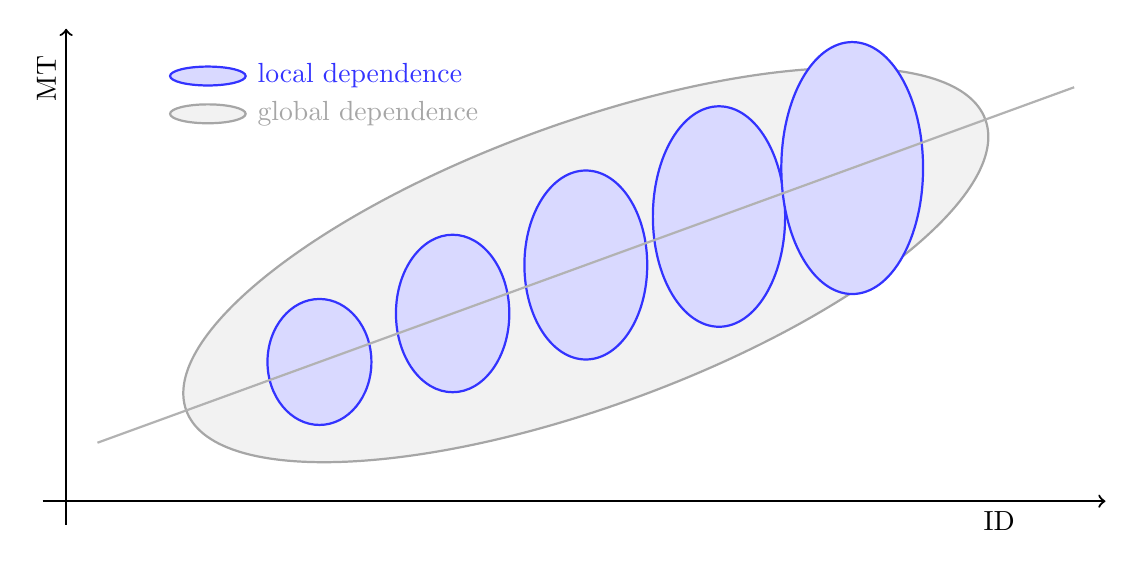
\begin{tikzpicture}[scale=1.2]

    % Define the angle of the alignment line
    \def\angle{20} % degrees
	\def\Eangle{20} % degrees

    % Draw the big background ellipse, rotated so that its major axis follows the line
    \draw[fill=gray!10, draw=gray!70, thick, rotate=\angle]
        (0,0) ellipse [x radius=4.5cm, y radius=1.5cm];

    % Define spacing and small ellipse sizes
    \def\spacing{1.5}
    \def\ry{1.0}
    \def\rx{0.3}

    % Draw 5 small ellipses whose centers are along a 20° line,
    % but each ellipse remains unrotated (aligned with x and y axes)
    \foreach \i in {-2,-1,0,1,2}{
        \pgfmathsetmacro{\x}{\i*\spacing*cos(\angle)}
        \pgfmathsetmacro{\y}{\i*\spacing*sin(\angle)}
		\pgfmathsetmacro{\currentRx}{(\i+3)/6 * \rx  + .5} % example
        \pgfmathsetmacro{\currentRy}{(\i+3)/6 * \ry + .5}
        \draw[fill=blue!15, draw=blue!80, thick]
            (\x,\y) ellipse [x radius=\currentRx cm, y radius=\currentRy cm];
    }
	\draw[fill=blue!15, draw=blue!80, thick] (-4,2) ellipse [x radius=.4 cm, y radius=.1 cm] node[right = .5cm, color=blue!80]{local dependence};
	\draw[fill=gray!10, draw=gray!70, thick] (-4,1.6) ellipse [x radius=.4 cm, y radius=.1 cm] node[right = .5cm, color=gray!70]{global dependence};
    
    % Optional: show the alignment axis
    % \draw[dashed, gray!60] (-7,0) -- (7,0);
    \draw[thick, gray!60, rotate=\Eangle] (-5.5,0) -- (5.5,0)
        node[right, black]{};
	\draw[thick, black, ->] (-5.5, -2.75) -- (-5.5, 2.5) node[rotate=90, pos=.9, above]{MT};
	\draw[thick, black, ->] (-5.75, -2.5) -- (5.5, -2.5) node[below, pos=.9]{ID};

\end{tikzpicture}

	\caption{The difference between the local and global dependency structure. The blue ellipses which represent 95\% confidence ellipses for data associated with one block, being oriented vertically, show no correlation between MT and \ide. The orange ellipsis, which represents the 95\% confidence ellipsis for the aggregated data, being oriented at an angle, shows that MT is correlated with \ide. This shows that data that is locally independent can still lead to dependencies when pooled across conditions. In this example, what causes the dependency is mostly the position of the means of the blue ellipses.}
	\label{fig:global_local_dep}
\end{figure}



% \begin{figure}[htbp]
% 	\centering
% 	\includegraphics[width=.8\textwidth]{tmp.pdf}
% 	\caption{The difference between the local and global dependency structure. The blue ellipses which represent 95\% confidence ellipses for data associated with one block, being oriented vertically, show no correlation between MT and \ide. The orange ellipsis, which represents the 95\% confidence ellipsis for the aggregated data, being oriented at an angle, shows that MT is correlated with \ide. This shows that data that is locally independent can still lead to dependencies when pooled across conditions. In this example, what causes the dependency is mostly the position of the means of the blue ellipses.}
% 	\label{fig:global_local_dep}
% \end{figure}

To estimate these joint distributions, we consider two complementary approaches.

\begin{enumerate}
	\item \textbf{Conditional EMG approach.}  
	We use the chain rule of probability:
	\begin{align}
		p(\mt, \ide | \D, \W, s) 
		&= p(\mt | \ide, \D, \W, s) \cdot{} p(\ide | \D, \W, s).
	\end{align}
	We then make the simplifying assumption that MT depends on task parameters only through \ide:
	\begin{align}
		p(\mt | \ide, \D, \W, s) = p(\mt | \ide).
	\end{align}
	This reduction avoids considering too many variables and uses the fact that \ide already summarizes task geometry and strategy \ie the remaining effect of s, \D and \W on MT are likely second order. 
	The conditional distribution of MT given \ide is modeled with the exponentially modified Gaussian (EMG) model described in \autoref{subs:rw::emg}. 
	We also model \(p(\ide | D, W, s)\) enabling the model to be used not just descriptively, but \textit{predictively}.
	Because the EMG has already been validated in prior work, our goal here is not to re-compare candidate models for $p(\mt|\ide)$. Instead, we focus on showing how the distinctive features that make the EMG model successful (asymmetry and quadratic variance) contribute to better fits, while placing greater emphasis on modeling $p(\ide| \D,\W,s)$ which has received less attention and is central to understanding SAT.
	
	\item \textbf{Copula-based approach.}  
	The EMG approach fixes the dependency structure between MT and \(ID_e\) through its quadratic variance model. 
	To allow more general forms of dependence, and thus study the SAT from a perspective that is agnostic to any form of dependence, we instead model the joint distribution using copulas, which capture the dependency between two variables independently of their marginals. 
	This approach removes the restriction imposed by the EMG variance model and provides a more flexible description of MT and \ide.
\end{enumerate}
\noindent Learning the global dependency \(p(\mt, \ide)\) proceeds analogously by dropping the conditioning on \D, \W, and $s$.
We apply these two modeling approaches to three datasets collected under progressively richer experimental protocols, moving from a classic Fitts' law task and a strategy-based task to a combined Fitts-with-strategy task.
\paragraph*{Study 1: Fitts protocol} 
In the first study (\autoref{sec:jgp}), we re-analyze data of a standard Fitts protocol (\autoref{background:protocols:fitts_protocol}), where accuracy is controlled by target width \W. 
Because this dataset was previously used to validate the EMG distribution by two independent works~\cite{gori2018these,zhao2022}, we focus here on copulas.
Several candidate copula models were considered to describe the global and local dependencies; the rotated Gumbel copula was selected as the best fit for the global distribution, capturing strong correlation in the lower tail. 
For the local distributions, a low-correlation Gaussian copula provided the best fit. 
A linear model relating \ide to ID is proposed to form the conditional distribution $p(\ide | \text{ID}, \D, \W)$. 
This study shows that the speed-accuracy tradeoff emerges globally, not locally.


\paragraph*{Study 2: Pure strategy protocol} 
In the second study (\autoref{sec:gop}), we analyze data from a pure strategy protocol (\autoref{background:protocols:guiard_protocol}), where accuracy is determined only by the participant's strategy $s$. 
As a first step, we examine the joint distribution of \mmt and \ide,  and propose a bivariate Gaussian model parametrized by $s$. 
% This model provides a bridge between Fitts' law, which collapses across all conditions, and full joint-distribution modeling, by capturing how \mmt and accuracy vary with strategy.
This simplified, aggregated view, highlights systematic effects of strategy on speed and accuracy without the additional variability present in single trials. This is important since unlike task parameters D and W, the influence of strategy alone on the speed-accuracy trade-off is less well modeled.
Thus, this preliminary analysis provides a new, simple model and provides a broad trend and some intuition for the more detailed analysis that follows.
Next, we show that the EMG model with quadratic variance also fits this dataset, extending its applicability. 
Finally, we find that the Gaussian and t-copulas provide the best fit for $p(\mt, \ide | s)$ and $p(\mt, \ide)$.
This study shows that user strategy directly shapes the dependency structure, highlighting the importance of modeling strategy explicitly.

\paragraph*{Study 3: Fitts-with-strategy protocol} 
In the third study (\autoref{sec:yamanaka}), we combine both approaches to manipulate accuracy, by analyzing data from a Fitts-with-strategy protocol (\autoref{background:protocols:full_protocol}), where accuracy is influenced by both target width \W and strategic instructions $s$. 
We model the local distribution $p(\mt, \ide | s, \D, \W)$, and confirm that the EMG with quadratic variance and asymmetric distribution provides good fits. 
As in the previous study, Gaussian and t-copulas yield the best joint models. 
We also extend the linear model relating \ide to ID by including a term for strategy. This extension makes explicit how strategy interacts with task difficulty to shape user accuracy, as captured through \ide.



\section{First study: Dependence between \ide and MT in Fitts' protocol\label{sec:jgp}}

\subsection{Dataset presentation}
We used an existing dataset by \citeauthor{jude2016}~\cite{jude2016} (JGP). The JGP dataset was generated using a 2D multi-directional tapping task~\cite{soukoreff2004} using the FittsStudy software~\cite{wobbrock2011}, with gestural interaction as input method. The experiment was replicated six times over three days, twice a day, for 15 participants with factors \W (64, 96, 128 (px)) and \D (256, 512, 1024, 1408 (px)) fully crossed, which makes 10 unique ID levels ranging from 1.52 to 4.58 bit. At 20 trials per block, the entire dataset consists of 21600 movements.
We noticed a bug in the dataset we downloaded, where the 2 last replications are identical to the two first, so we discarded the 2 last replications from the dataset, leaving us with 4 replications (14400 trials remaining). The JGP dataset is pre-processed; \ide and MT are already calculated. 




% \subsection{Measures of association between \ide and MT}
% For each participant and each replication, we computed Pearson's $r$, Spearman's $\rho$ and Kendall's $\tau$. Histograms of the three measures are provided \autoref{fig:association}, where we notice values typically associated with moderately/strong (rank) correlation. We also computed intraclass correlation coefficients (ICC), which are all significant at the $\alpha=0.011$ level (results available in the supplementary materials), strongly suggesting individual differences in association.
% Hence, the JGP dataset pictures moderately strong correlations between MT and \ide for all participants, and differences between participants. We looked at the association between \ide and MT; although there seemed to be a small negative effect of W, with larger values of W leading to lower associations, this effect was not statistically significant ($\alpha > 0.05$). The fits can be found in the supplementary materials.
% \begin{figure}[htbp]
% 	\centering
% 	\includegraphics[width=.5\textwidth]{img/association.pdf}
% 	\caption{Histogram of the measures of association (Pearson's $r$, Spearman's $\rho$ and Kendall's $\tau$).}
% 	\label{fig:association}
% 	\Description{Histogram of the measures of association (Pearson's $r$, Spearman's $\rho$ and Kendall's $\tau$).}
% \end{figure}

\subsection{Fitting EMG on MT given \ide values \label{subs:jgp:emg}}
We fitted the EMG model for each participant and for each replication. In line with existing works on this dataset~\cite{gori2018these,zhao2022}, the EMG fit was largely superior to the Gaussian fit obtained via linear regression. We namely found AIC differences routinely above 300; typically a difference of 10 is already considered strongly discriminative. A pair-plot of the fitted parameters can be found in the supplementary materials.

% are displayed \autoref{fig:pairplot_emg_jgp}. We notice that
% \begin{itemize}
% 	\item $\beta_0$ and $\beta_1$ are strongly negatively correlated. This suggests that Fitts' \textit{min} law tends to pivot | larger intercepts make the slope become more horizontal and thus smaller.
% 	\item The constant variance term $\lambda_0$ is very often null
% 	\item $\lambda_1$ is always positive, in line with the increasing variance hypothesis.
% \end{itemize}

% \begin{figure}[htbp]
% 	\centering
% 	\includegraphics[width=.8\textwidth]{img/pairplot_emg_jgp.pdf}
% 	\caption{<caption>}
% 	\label{fig:pairplot_emg_jgp}
% \end{figure}


\subsection{Fitting copulas on (MT, \ide) \label{sub:jgp::fit_copula}}

\subsubsection{Local dependency structure}
To test whether the SAT appears within individual task conditions, we examined the local dependency between MT and \ide through $p(\mt, \ide | \D, \W)$. If the SAT held locally, one would expect systematic dependence between the two variables when D and W are fixed. 

We compared candidate copula models using the model evidence ratio $\mathcal{R}$ as explained in \autoref{app:copula:compare}. This ratio expresses how likely one model is relative to the best-fitting model: for example, $\mathcal{R}=0.1$ means the model is about 10 times less likely to be the true model than the current best fitting. This allows us to compare copulas on a common scale.


Pooled over participants and across D$\times$W pairs, the independent copula was most often selected as the best-fitting model (see %\autoref{fig:copula_fit_jgp_dwp}, 
\autoref{fig:copula_fit_jgp_dw}). This indicates that within a given condition, longer movement times were not reliably associated with higher effective difficulty. In other words, the local dependency between MT and \ide was weak or absent. 

An exception occurred for the smallest target condition ($\W=64$), where both Spearman's $\rho$ and Kendall's $\tau$ correlations were slightly negative. This suggests that in this extreme case, faster movements could even be associated with greater accuracy, the opposite of the expected SAT. While weak, this paradoxical result highlights that the large trial-to-trial variability can obscure or even invert the trade-off locally.

These findings suggest that the SAT is not strongly expressed at the local level, where performance appears largely independent once task parameters are fixed.

% \begin{figure}[htbp]
% 	\centering
% 	\includegraphics[width=.8\textwidth]{img/model_evidence_ratio_DW_jgp}
% 	\caption{Model evidence ratio $\mathcal{R}$ computed against the best copula for each D$\times$W pair and each participant.}
% 	\label{fig:copula_fit_jgp_dwp}
% \end{figure}



\begin{figure}[htbp]
	\begin{subfigure}[c]{.48\textwidth}
	\centering
	\includegraphics[width=\textwidth]{img/R_DW.pdf}
	\caption{Model evidence ratios ($\mathcal{R}$) for pooled participant data across D$\times$W conditions. Except for the smallest target condition ($W=64$), the independent copula provided the best fit, indicating no consistent local dependency between MT and \ide. $\mathcal{R}=0.1$ means the model is about 10 times less likely than the best-fitting copula.}
	\label{fig:copula_fit_jgp_dw}
	\end{subfigure}
	\hfill
	\begin{subfigure}[c]{.48\textwidth}
	\centering
	\includegraphics[width=\textwidth]{img/model_evidence_ratio_jgp.pdf}
	\caption{Model evidence ratios $\mathcal{R}$ for global copula fits across participants. The rotated Gumbel copula and Galambos copulas consistently outperformed other candidates.}
	\label{fig:copulas_jgp}
	\end{subfigure}
	\caption{Copula comparisons for the JGP dataset.}
	
\end{figure}

% \begin{figure}[htbp]
% 	\centering
% 	\includegraphics[width=.5\textwidth]{img/R_DW.pdf}
% 	\caption{Model evidence ratios ($\mathcal{R}$) for pooled participant data across D$\times$W conditions. Except for the smallest target condition ($W=64$), the independent copula provided the best fit, indicating no consistent local dependency between MT and \ide. $\mathcal{R}=0.1$ means the model is about 10 times less likely than the best-fitting copula.}
% 	\label{fig:copula_fit_jgp_dw}
% \end{figure}


\subsubsection{Global dependency structure}
We then turned to the global dependency $p(\mt, \ide)$, pooling data across task conditions. In contrast to the local case, and as expected, we found clear evidence of dependence between MT and \ide. 

The rotated Gumbel copula consistently provided the best fit across participants (\autoref{fig:copulas_jgp}). This model captures strong lower-tail dependence, meaning that low MT values align closely with low \ide values. This means that when tasks are easier, movements are faster and much more consistent; as tasks become more difficult, variability in MT increases and the relationship between \ide and MT weakens. The rotated Galambos copula was the second-best model, this can likely be explained by the fact that for some parameter values it is extremely similar to the rotated Gumbel~\cite{genest2017},

Together, these results show a contrast: while the SAT is weak at the local level, it emerges clearly in the global distribution once conditions are aggregated.

% \begin{figure}[htbp]
% 	\centering
% 	\includegraphics[width=\textwidth]{img/model_evidence_ratio_jgp.pdf}
% 	\caption{Model evidence ratios $\mathcal{R}$ for global copula fits across participants. The rotated Gumbel copula and Galambos copulas consistently outperformed other candidates.}
% 	\label{fig:copulas_jgp}
% \end{figure}




% ******
% \subsection{Fitting copulas on (MT, \ide) \label{sub:jgp::fit_copula}}




% \subsubsection{Local dependency structure}
% We first examined the local dependency between \ide and MT through $p(\mt, \ide | \D, \W)$. We fitted copulas to the pointing data for each participant and (D, W) pair separately as detailed in \autoref{app:copula:fit}. The comparison of copulas was based on the model evidence ratio $\mathcal{R}$ explained \autoref{app:copula:compare}. The interpretation of $\mathcal{R}$ is as follows: when comparing two models with an evidence ratio of $x$, there is 1 chance out of $1/x$ that the worst model is actually better than the other.
% The t-EV, t, rotated Gumbel, rotated Galambos, and rotated HR copulas often failed to converge.\footnote{This can happen when a copula is made to fit a dependency structure it can't represent, \eg fitting a copula which can only model positive rank correlation to a dataset with negative rank correlation.} Because these failures to converge were spread equally across (D,W) pairs (see the supplementary materials), we simply excluded these copulas from the analysis. 


% The $\mathcal{R}$ values for the remaining copulas and D$\times$W condition pairs are shown in \autoref{fig:copula_fit_jgp_dwp}. The Gaussian copula emerged as the best fit according to $\mathcal{R}$, while the Galambos, HR, and Clayton copulas also provided reasonable dependence models under certain conditions.
% We did not observe any relationship between the D and W conditions and the best-fitting copula, which suggests that the structure of the dependence between \ide and MT is influenced by D or W. 

% Considering the analysis was performed for each participant and each D,W pair, there are only four distinct \ide levels, which usually are quite close to one another. Thus, to get more reliable data, we pooled the participant data together before fitting the copulas and re-analyzing them for different (D,W) conditions, the interpretation being that we look at population version of $p(\mt, \ide | \D, \W)$. Again, we had to remove the following copulas from the analysis: Galambos, HR, t-EV, rotated Galambos, and rotated HR. Surprisingly, as illustrated \autoref{fig:copula_fit_jgp_dw} we found that the independent copula was the best fitting copula, except for the $\W=64$ condition. This means that except for the smallest target, there is no evidence for a local dependence between MT and \ide \ie for a given (D,W) pair, a larger \ide is not associated with larger MT values. For completeness, we computed rank correlations for each condition; for the 4 different conditions where $\W=64$, both Spearman's and Kendall's rank correlation between \ide and MT actually turned out slightly negative, which would indicate higher speeds are associated to higher accuracy, opposite to the speed-accuracy tradeoff.


% \begin{figure}[htbp]
% 	\centering
% 	\includegraphics[width=.8\textwidth]{img/model_evidence_ratio_DW_jgp}
% 	\caption{Model evidence ratio $\mathcal{R}$ computed against the best copula for each D$\times$W pair and each participant.}
% 	\label{fig:copula_fit_jgp_dwp}
% \end{figure}


% \begin{figure}[htbp]
% 	\centering
% 	\includegraphics[width=.7\textwidth]{img/R_DW.pdf}
% 	\caption{Model evidence ratio $\mathcal{R}$ computed against the best copula for each D$\times$W pair, pooled over participants.}
% 	\label{fig:copula_fit_jgp_dw}
% \end{figure}


% \subsubsection{Global dependency structure}
% The previous analysis suggest that there is little to no local dependency structure between MT and \ide. We thus examined the global dependency between \ide and MT by fitting $p(\mt, \ide)$ with the same method as before.

% The results displayed \autoref{fig:copulas_jgp} show that the rotated Gumbel copula consistently outperformed other models. The rotated Galambos copula followed closely | under certain conditions the Gumbel and Galambos copulas are known to be very similar~\cite{genest2017} which explains this observation. 


% \begin{figure}[htbp]
% 	\centering
% 	\includegraphics[width=\textwidth]{img/model_evidence_ratio_jgp.pdf}
% 	\caption{Model evidence ratio $\mathcal{R}$ computed against the best copula for each participant, with a threshold at $\mathcal{R} = 1e^{-4}$ for a better use of the color palette. The interpretation of $\mathcal{R}$ is as odds against the best fitting copula: For example, a model with $\mathcal{R} = 0.11$ indicates that the best model is about $1/0.11 \simeq 9$ times more likely.}
% 	\label{fig:copulas_jgp}
% 	\Description{Log-likelihoods for each copula and for each participant. Closest to 1 (greenest) indicated best fit. The log-likelihoods are the result of averaging the log-likelihoods of the 4 replications. They are then normalized for each participant by dividing the log-likelihood by the maximum log-likelihood over all potential copulas.}
% \end{figure}


\subsection{Model between \ide and D, W, ID\label{sub:jgp_id}} 
To test whether W and D influence \ide beyond their joint contribution through ID, we fitted four linear mixed-effects models (LMM) with random intercepts for participants (see \autoref{app:lmm} for an explanation of LMM and how they were fitted and compared): a full model with ID, W, D, and all interactions, two simpler models with only ID+W or ID+D, and a baseline with ID alone.
A summary of the results are displayed \autoref{tab:fit_jgp_ide_id}, while the full fits are available in the supplementary materials.


The full model is difficult to interpret due to collinearity between ID, W, and D, and model comparison shows that it was not supported relative to simpler alternatives, so it was excluded. The simpler models revealed a clear effect of D: both its main effect and its interaction with ID were significant ($\alpha=0.05$), while W showed no significant contribution. Log-likelihoods for the D and W models were essentially equivalent. The ID-only model was rejected based on significantly lower log-likelihood.
The two simple model fits are shown in \autoref{fig:ide_id_jpg}, which illustrates that D significantly shifts the \ide - ID relationship upwards. This is concistent with general results in psychophysics where longer distances lead to overall larger variability in movement trajectories. 
This result diverges from \citeauthor{zhai2004nominal}~\cite{zhai2004nominal}, who reported W effects\footnote{\autoref{fig:ide_id_jpg} suggests an effect of W on the slope of the \ide-ID relation, but this effect did not turn out significant}. Two factors may explain the discrepancy. First, our W values (64--128 px) were larger than theirs (12--72 px), and W-ID interactions likely manifest more strongly at smaller target sizes.\footnote{However, comparisons must be taken cautiously, since pixels alone do not tell the full story, we also have to consider display density and input device characteristics \cite{casiez2011}.} Second, fully disentangling W or D from ID requires a shape-scale design \cite{gori2018chi, guiard2009}, which was the case of this dataset.
Overall, the additional effects of D and especially W beyond ID, while they can be of theoretical interest under specific experimental designs, are likely negligible in most practical contexts.



\begin{figure}[htbp]
	\centering
	\includegraphics[width=\textwidth]{img/ide_id_jpg.pdf}
	\caption{The relationship between \ide and ID depending on W values (left) and D values (right). The filled circles represent the observed \ide values for prescribed ID levels for varying W or D values, while the lines represent the linear model fits for varying W or D values. This suggests small effects on slope and intercept of both W and D.}
	\label{fig:ide_id_jpg}
\end{figure}


\begin{table}
	\caption{Mixed effect model fit results for four different models of \ide, expressed in R-style formula syntax. The estimated coefficients are displayed associated with their p-value (in bold if p<0.05). The last line displays the log-likelihood of the model (higher indicates better fit).}
	\label{tab:fit_jgp_ide_id}
\begin{center}
	\begin{tabular}{lrrrrrr}
	\hline
		  &  $\text{ID}*\W*\D + (1|\text{Participant})$ & $\text{ID}*\W + (1|\text{Participant})$ & $\text{ID}*\D + (1 | \text{Participant})$ & $\text{ID}+ (1 | \text{Participant})$  \\
	\hline
	Intercept &  0.262 (p=0.402) &    				0.016 (p=0.833) &  0.1 \textbf{(p=0.016)} & 0.079 \textbf{(p\textless0.001)} \\
	ID        &  0.846 \textbf{(p\textless0.001)} &    0.918 (\textbf{p\textless0.001}) &  0.890 (\textbf{p\textless0.001}) & 0.937 \textbf{(p\textless0.001)}  \\
	w         & -0.992 (p = 0.589) & 0.162 (p=0.827)    &   & \\
	ID:w      & -0.664 (p=0.763) &    0.379 (p=0.102)  &   & \\
	D         &  0.593 (p=0.707) &    &  0.296 (\textbf{p\textless0.001})  & \\
	ID:D      & -0.042 (p=0.837) &     & -0.040 (\textbf{p=0.025})  & \\
	w:D       &  5.022 (p=0.389) &     &  &   \\
	ID:w:D    & -1.378 (p=0.429) &     &   & \\
	log-likelihood & 401 & 401 & 401  & 380\\
	\hline
	\end{tabular}
	\end{center}
	\end{table}


% To evaluate the effects W and D can have on \ide other than through ID, we fitted\footnote{See \autoref{app:lmm}} four mixed-effects linear models incorporating main and interaction terms, each with a random intercept for participants:
% \begin{align}
% 	\ide & \sim \text{ID}*\W*\D + (1|\text{Participant}) \label{eq:melr_full}\\
% 	\ide & \sim \text{ID}*\W + (1|\text{Participant}) \label{eq:melr_w}\\
% 	\ide & \sim \text{ID}*\D + (1 | \text{Participant}) \label{eq:melr_d} \\
% 	\ide & \sim \text{ID}+ (1 | \text{Participant}) \label{eq:melr_id}
% \end{align}
% The full model (\autoref{eq:melr_full}) includes seven terms: three main effects, three pairwise interactions, and one three-way interaction. However, since ID is a function of both D and W, the model has highly correlated predictors, which complicates interpretation of the 8 coefficients. Therefore, we also examined simpler models (\autoref{eq:melr_w} and \autoref{eq:melr_d}).
% The fits of the simpler models are shown in \autoref{fig:ide_id_jpg}, where we observe:

% \begin{itemize}
% 	\item \textbf{W's Effect:} A slight slope reduction as W decreases, suggesting a positive interaction between W and ID. This aligns with \autoref{subs:background::target_util}, where smaller W values prompt over-utilization of the target, leading to smaller \ide values.
% 	\item \textbf{D's Effect:} Both slope and intercept increase with larger D, indicating higher overall \ide values.
% \end{itemize}


% Detailed summaries of the fitted models are provided in the supplementary materials and summarized \autoref{tab:fit_jgp_ide_id}. The key findings are:
% \begin{itemize}
% 	\item In the full model (\autoref{eq:melr_full}), only ID has a significant effect ($\alpha = 0.05$). However, multicollinearity likely hampers the separate evaluation of D, W, and ID effects. Further, model comparison based on likelihood does not support this model (the simpler models achieve the same likelihood with less free parameters).
% 	\item In the simpler models:
% 		\begin{itemize}
% 			\item D and its interaction with ID are significant ($\alpha=0.05$) contributors to \ide.
% 			\item W and its interaction with ID are not significant ($\alpha=0.05$) contributors to \ide.
% 		\end{itemize}
% \end{itemize}

% Log-likelihood comparisons show that the full model's log-likelihood is within one point of the two simpler models (\autoref{eq:melr_w} and \autoref{eq:melr_d}), despite the former having twice as many fixed effect parameters.  Consequently, complexity-penalizing criteria (e.g., AIC, BIC) favor the simpler models. The model with only ID as main effect scores much lower on likelihood, and is therefore not supported by the data.

% In conclusion, while the visual fits suggested a significant effect of W on the slope of the (\ide, ID) relationship, this was not confirmed by statistical analysis. On the other hand, the effect of D was found to be significant, and the D model \autoref{eq:melr_d} was equivalent from a likelihood perspective.  This finding diverges from earlier results by Zhai \etal~\cite{zhai2004nominal}. Two possible explanations are:
% \begin{itemize}
% 	\item The values of W in this experiment (64, 96, 128)px were larger than in~\cite{zhai2004nominal} (12, 36, 72)px\footnote{Comparisons based on pixel sizes only are not necessarily meaningful, as they are only equivalent under identical pixel densities, and from a motor control perspective, also depend on various properties of the input device~\cite{casiez2011}.}; The interaction between W and ID likely would likely manifest itself more for small values of W.
% 	\item Evaluating a model like \autoref{eq:melr_w} would benefit from a fully crossed ID and W design, such as a shape $\times$ scale design~\cite{gori2018chi, guiard2009} to break the collinearity between ID and W (similar reasoning can be applied to the collinearity between ID and D).
% \end{itemize}


% \begin{figure}[htbp]
% 	\centering
% 	\includegraphics[width=\textwidth]{img/ide_id_jpg.pdf}
% 	\caption{The relationship between \ide and ID depending on W values (left) and D values (left). The filled circles represent the observed \ide values for prescribed ID levels for varying W or D values, while the lines represent the linear model fits for varying W or D values.}
% 	\label{fig:ide_id_jpg}
% \end{figure}


% \begin{table}
% 	\caption{Mixed effect model fit results for \autoref{eq:melr_full}, \autoref{eq:melr_w} and \autoref{eq:melr_d}. Each line (except the last, which displays the log-likelihood associated with each model) displays the estimated coefficient associated with the variable in the left column as well its associated p-value (in bold if p<0.05).}
% 	\label{tab:fit_jgp_ide_id}
% \begin{center}
% 	\begin{tabular}{lrrrrrr}
% 	\hline
% 			  &  Full model (\autoref{eq:melr_full}) & W model (\autoref{eq:melr_w}) &  D model (\autoref{eq:melr_d}) & only ID (\autoref{eq:melr_id})  \\
% 	\hline
% 	Intercept &  0.262 (p=0.402) &    				0.016 (p=0.833) &  0.1 \textbf{(p=0.016)} & 0.079 \textbf{(p\textless0.001)} \\
% 	ID        &  0.846 \textbf{(p\textless0.001)} &    0.918 (\textbf{p\textless0.001}) &  0.890 (\textbf{p\textless0.001}) & 0.937 \textbf{(p\textless0.001)}  \\
% 	w         & -0.992 (p = 0.589) & 0.162 (p=0.827)    &   & \\
% 	ID:w      & -0.664 (p=0.763) &    0.379 (p=0.102)  &   & \\
% 	D         &  0.593 (p=0.707) &    &  0.296 (\textbf{p\textless0.001})  & \\
% 	ID:D      & -0.042 (p=0.837) &     & -0.040 (\textbf{p=0.025})  & \\
% 	w:D       &  5.022 (p=0.389) &     &  &   \\
% 	ID:w:D    & -1.378 (p=0.429) &     &   & \\
% 	log-likelihood & 401 & 401 & 401  & 380\\
% 	\hline
% 	\end{tabular}
% 	\end{center}
% 	\end{table}


		
					

\subsection{Interpretation of the first study \label{study_one:interpretation}}
This study examined dependencies between \ide and MT under Fitts' protocol, where accuracy is imposed by target width W. At the local level, copula fits showed little to no correlation between \ide and MT within a given condition, with the smallest target size even yielding a slight negative correlation. This suggests that, when accuracy is specified a priori, movements within a fixed (D,W) pair are essentially equivalent with respect to the SAT: variability in execution reflects motor noise more than systematic planning trade-offs.
The analysis at the global level revealed a clear dependence, showing that the SAT only emerges across task conditions. The dependence was best captured by the rotated Gumbel copula, which emphasizes lower-tail dependence. This implies a strong correlation between low values of \ide and MT \ie a small spread of the MT data for low values of \ide, which is consistent with the quadratic variance model used in the EMG model.
Finally, we analyzed the relationship between \ide and ID. Possible D and W effects were weak, and not always significant, but could have been misestimated due to collinearity between D, W and ID. Thus, to adress these collinearity issues, we fit the linear models with ridge regression with cross-validation\footnote{Ridge regression is a technique for fitting linear models when collinearity exists among predictors, as it produces more stable and reliable estimates of effects~\cite{gruber2017}. The method introduces a regularization term controlled by a hyperparameter known as the ridge parameter. When the ridge parameter is set to 0, ridge regression reduces to the traditional ordinary least squares approach. As the ridge parameter increases, the method progressively shrinks the variance of the coefficient estimates, improving stability and reducing sensitivity to multicollinearity. The optimal value of the ridge parameter is determined through cross-validation.}. Although detailed results are not reported here, the estimated coefficient for ID was 0.94 \ie closer to 1 than the estimates from the presented linear models. This suggests that the presented effects of D and W are actually slightly inflated by collinearity. Thus, this further supports that ID is the dominant predictor for \ide, and that additional effects of D and W are negligible.


\section{Second study: Dependence between \ide and MT in the pure strategy protocol \label{sec:gop}}
In the pure strategy protocol (see \autoref{background:protocols:guiard_protocol}), accuracy is not manipulated by W but by the experimenter instructing the user to conform to strategies favoring speed or accuracy. 

\subsection{The GO dataset}
We investigate the effect of participant strategy on movement time and \ide, using the Guiard-Olafsdottir (GO) dataset~\cite{guiard2011}.
Participants had to aim at a line (1D task), with five different strategies, from speed emphasis allowing a large spread of endpoints, to precision emphasis where the goal is to target the 1-pixel-wide line. 
%The balanced condition represents a somewhat natural strategy \ie how the participant would operate had no instructions been given. 
For comparison, the instruction in a standard Fitts experiment is usually between the \textit{speed} and \textit{balanced} condition, depending on the experimenter.
The 16 participants performed 5 strategies, each replicated 5 times. We thus have 25 blocks per participant, each of about 15 to 20 movements each. 
We used a pre-processed version of the dataset used in~\cite{gori2020}. One participant had partially corrupt data; we removed this participant entirely for safety. We also removed 79 outlier points, given the recording procedure was sometimes unreliable. The resulting dataset is composed of $15 \times 5 \times 5 = 375$ different experimental blocks for a total of 5858 movements.

% \subsection{Association per strategy}
% We computed association measures for the GO dataset, per strategy, and per participant. The figures are available in the supplementary materials, and are not reproduced here: $r$, $\rho$ and $\tau$ have average values close to 0, with large spread (values between -0.5 and + 0.5); we consider the results to be too noisy to be meaningful.



\subsection{A model between \mmt and \ide parametrized by strategy}

\paragraph{Correlation between \ide and \mmt and conformity with Fitts' law}
A summary of the GO dataset, shown in \autoref{fig:fittslaw_guiard} confirms that data from the pure strategy protocol conforms with Fitts' law (\autoref{eq:ide}). Participants covered a wide range of \ide (1 to 9 bits), depending on the strategy.
While aggregating data per strategy yields a very high correlation between \mmt and \ide ($R^2=0.97$), block-level averages show more variability ($R^2=0.58$)\footnote{It is usual to report very high values of $R^2$ in Fitts law evaluations, but this is for a large part due to the practice of aggregating and averaging data, which masks the actual data's variability~\cite{gori2018chi,drewes2013}.}.
To capture how strategy affects behavior without overly masking this variability, we first model \mmt conditional on strategy. This provides a simple model of strategic effects, useful for simulation and prediction, and helps to build intuition for the subsequent trial-by-trial analysis.


\paragraph{A bivariate Gaussian model for \mmt and \ide for each strategy}
To characterize how each strategy affects MT and accuracy, we fit a bivariate Gaussian to the observed (\mmt, \ide) data for each of the five strategies in the GO dataset:
\begin{align}
	\begin{pmatrix}
		\ide \\
		\mmt
	\end{pmatrix} \sim \mathcal{N} \left( \begin{bmatrix}
			                                      \mu_i \\
			                                      \mu_t
		                                      \end{bmatrix}, \begin{bmatrix}
			                                                     \sigma^2_i          & r \sigma_i \sigma_t \\
			                                                     r \sigma_i \sigma_t & \sigma_t^2
		                                                     \end{bmatrix} \right) \label{eq:gaussian_ide_mt}
\end{align}
where $\mu_i$, $\sigma_i^2$ are the mean and variance of \ide, $\mu_t$ and $\sigma_t^2$ those of \mmt, and $r$ the Pearson correlation. 
We chose the bivariate Gaussian model because it is simple, easy to interpret, symmetric, and it makes the dependence between \mmt and \ide completely specified via a single parameter (Pearson's $r$), which facilitates analysis.
The conditional mean of MT given \ide is linear:
\begin{align}
	\mathbb{E}[\mmt | \ide] = \mu_t + r \frac{\sigma_i}{\sigma_t}(\ide - \mu_i).  \label{eq:mmt_ide_gauss}
\end{align}
which, in line with Proposition~\ref{prop}, ensures that, at the level of strategy, the model is consistent with Fitts' law while still capturing variability in both MT and \ide.




The bivariate Gaussian fits for each strategy in the GO dataset are displayed in \autoref{fig:go_ide}. Each ellipse shows the $95\%$ prediction region of a bivariate Gaussian fitted to (\ide,\mmt). The separation of ellipses reflects overall differences between strategies, while their orientation shows the local correlation between \ide and \mmt\footnote{The covariance matrix of a Gaussian bivariate is the rightmost term of \autoref{eq:gaussian_ide_mt} where $\rho$ is the correlation between the two components. The angle of the prediction ellipsis is given by $\frac{1}{2} \arctan \left( \frac{2\rho \sigma_i\sigma_t}{\sigma_i^2 - \sigma_t^2} \right) $.}. Strategies produce higher means and larger spreads with consistent positive correlation, whereas the \textit{speed emphasis} condition shows little to no correlation.%: when participants emphasize speed above anything else, accuracy actually becomes independent of local changes in speed, which is consistent with purely feedforward movements~\cite{gan1988, crossman1957}.


\begin{figure}[htbp]
   \centering
   \begin{subfigure}[t]{0.47\textwidth}
	   \includegraphics[width=\linewidth]{img/fittslaw_guiard.pdf}
	\caption{Fitts' law evaluated on the GO dataset. Each point summarizes data from one block, where color indicates participant strategy, the diamonds represent average movement time and \ide aggregated across all participants for each strategy. $r^2(\ide, \mmt)$ is very close to 1 when considering aggregates (orange), but is otherwise considerably lower.}
	\label{fig:fittslaw_guiard}
   \end{subfigure}
   \hfill
   \begin{subfigure}[t]{0.505\textwidth}
	   \includegraphics[width=\linewidth]{img/fitts_ide_go_with_ellipse.pdf}
	\caption{Gaussian fits for each strategy in the GO dataset. Each ellipse shows the $95\%$ prediction region of a bivariate Gaussian fitted to (\ide,\mmt). The separation of ellipses reflects overall differences between strategies, while their orientation shows the local correlation between \ide and \mmt. Strategies oriented toward precision produce higher means and larger spreads with consistent positive correlation, whereas the \textit{speed emphasis} condition shows little to no correlation.}
	\label{fig:go_ide}
   \end{subfigure}
  
\caption{Fitts' law and the bivariate Gaussian model compared on the GO dataset.}
\label{fig:main}
\end{figure}


\begin{figure}[htbp]
	\centering
	
\end{figure}





\begin{figure}[htbp]
	\centering
	
\end{figure}



\paragraph{Strategy Dependent Bivariate Gaussian model for \mmt and \ide}
We combined the five strategy-specific Gaussian fits into a single model by assigning each strategy a numerical score on [-1,1] where -1 stands for complete speed emphasis, 0 for balanced, and +1 for complete precision emphasis. This simple symmetric coding allows us to examine how the Gaussian parameters vary with strategy, without relying on post-hoc measures such as \ide. The model parameters are represented as function of coded strategy in \autoref{fig:meancov_strat}. We further compared linear models of each Gaussian parameter against constant (no-effect) models using AIC (\autoref{tab:aic_gop}). It results in three distinct cases:
\begin{enumerate}
	\item Both $\mu_i$ and $\mu_t$ increase linearly with strategy, with strong statistical support. This captures the intuitive shift from faster but less precise movements under speed emphasis to slower, more precise movements under precision emphasis.
	\item The spreads ($\sigma_i$, $\sigma_t$) show weaker trends. For $\sigma_i$, the constant model was favored overall, but the speed condition was a clear outlier. For $\sigma_t$ evidence slightly favored a linear increase.
	\item The correlation $r$ is best described as constant across strategies, except for the speed emphasis condition where it collapsed toward zero. In other words, under speed emphasis, accuracy decouples from mean movement time.
\end{enumerate}

% We can unite the five models into a single one by representing strategy numerically rather than ordinally. We thus map the five instructions to equally spaced points on the interval [-1,1]\footnote{The choice here may seem naïve, and we could have mapped strategy to the set of real values via \ide. However, our choice has two advantages: the mapping can be defined before movements are performed, and does not depend on each participant.}, with 0 as the balanced strategy, -1 for speed emphasis, and 1 for precision emphasis. We then assessed how the five parameters of the bivariate Gaussian model \autoref{eq:gaussian_ide_mt} aligned with this numerical strategy, by fitting a linear model on each parameter. 
% First, we determined whether to consider the linear model
% \begin{align}
% 	\text{X} \sim \text{strategy (strategy model)}
% \end{align}
% or the simpler constant model ($\text{X} \sim 1$) based on AIC comparisons reported \autoref{tab:aic_gop}, where $X$ represents any of the 5 parameters of \autoref{eq:gaussian_ide_mt}.


\begin{table}[htbp]
	\centering
	\caption{Comparison between models with or without a strategy main effect, for $\mu_i$, $\mu_t$, $\sigma_i$, $\sigma_t$, $\rho$. The table gives the AIC for each model fit; lower is better and differences of about 10 indicate substantial support for the lower AIC model. The AIC in bold signals this was identified as the best model. When the AIC difference was below 5, the simpler model was selected.}
	\label{tab:aic_gop}
	\begin{tabular}{c rr}
	parameter of \autoref{eq:gaussian_ide_mt}	 & strategy model AIC & constant model AIC\\
	$\mu_i$ &  \textbf{1} & 21 \\
	$\mu_t$ & \textbf{-4} & 9 \\
	$\sigma_i$ & 1 & \textbf{3} \\
	$\sigma_t$ & \textbf{-17} & -10 \\
	$\rho$ &  -3& \textbf{1} \\
	\end{tabular}
\end{table}
% We then fitted the models, displayed \autoref{fig:meancov_strat}. We observe that:
% \begin{itemize}
% 	\item The linear increase of the mean ($\mu_i$, $\mu_t$) with numerical strategy is visually clear, and supported by high goodness of fit ($r^2$) and large AIC differences.
% 	\item The increase of $\sigma_i$ and $\sigma_t$ with numerical strategy could also reasonably be described by a linear model, although evidence is less strong than for the mean. For $\sigma_i$, AIC comparison suggested the simpler constant model. Note that the value of $\sigma_i$ for the \textit{speed emphasis} condition differs strongly from the others; the mean $\sigma_i$ without the \textit{speed emphasis} condition is $\sigma_i = 1.19$. For $\sigma_t$, the AIC difference between the linear and constant model was slightly below 10 (7); we decided to consider the linear model to have an estimate of the effect size of strategy.
% 	\item For $\rho$, model comparison suggested the constant model. Still, one sees that the speed emphasis condition is quite different from the others. As alternate model we considered $r=0$ for the \textit{speed emphasis} ($s=-1$) condition, and a constant correlation for the other conditions; we computed the mean $r$ for the 4 other conditions and obtained $r=0.44$.
% \end{itemize}

Crucially, the linear dependence of $\mu_i$ and $\mu_t$ on strategy implies that their relationship is itself linear, reproducing a Fitts-like law across strategies:


\begin{align}
	\mu_i & = \alpha' + \beta'\,s  \longrightarrow s =  \frac{\mu_i - \alpha'}{\beta'} \\
	\mu_t & = \alpha + \beta\,s = \alpha + \frac{\beta}{\beta'} (\mu_i - \alpha')  = \alpha - \frac{\beta}{\beta'}\alpha' + \frac{\beta}{\beta'}\mu_i,
\end{align}

Thus, the Gaussian model is compatible both with local Fitts' law (within a given strategy, via \autoref{eq:mmt_ide_gauss}) and with global Fitts' law (across strategies, via the linear trend in means). The model therefore provides a bridge between individual strategies and Fitts' law.
% The linear relationship of $\mu_i$ and $\mu_t$ on $s$ makes the obtained model consistent with Fitts' law (globally) across strategies since
% \begin{align}
% 	\mu_i & = \alpha' + \beta'\,s  \longrightarrow s =  \frac{\mu_i - \alpha'}{\beta'} \\
% 	\mu_t & = \alpha + \beta\,s = \alpha + \frac{\beta}{\beta'} (\mu_i - \alpha')  = \alpha - \frac{\beta}{\beta'}\alpha' + \frac{\beta}{\beta'}\mu_i,
% \end{align}
% which conforms with our finding in \autoref{fig:fittslaw_guiard}. Thus, the Gaussian bivariate model is consistent with the local Fitts' law (within a strategy) and the linear model for $\mu_i$ and $\mu_t$ is consistent with the global Fitts' law (across strategies). Note that the slopes and intercepts of each local Fitts' law are different, and different from the slopes and intercepts of the global Fitts' law, as on can guess in \autoref{fig:go_ide}, and since the parameters of \autoref{eq:mmt_ide_gauss} depend on $s$.



% We return to \autoref{eq:mmt_ide_gauss} to consider whether it is also compatible with Fitts' law across strategy.
% The linear models for $\mu_i$ and $\mu_t$ are evident fits, which gives
% \begin{align}
% 	\mathbb{E}[\mmt | \ide, s] = \alpha + \beta\,s + r\frac{\sigma_
% 	i}{\sigma_t} (\ide - \alpha' - \beta''\,s).
% \end{align}
% If the product term $r\frac{\sigma_i}{\sigma_t}$ were constant, then we would obtain 
% \begin{align}
% 	\mathbb{E}[\mmt | \ide, s] = \alpha + \beta\,s + k(\ide - \alpha' - \beta''\,s) = p_1 + p_2\ide + p_3 \,s.
% \end{align}

\begin{figure}[htbp]
	\centering
	\makebox[\textwidth]{
		\includegraphics[width=1.2\columnwidth]{img/mean_cov_strat.pdf}
	}
	\caption{The parameters of the mean and covariance of the bivariate Gaussian model defined in \autoref{eq:gaussian_ide_mt} plotted against the five numerical strategies. The associated linear fits that result from the model selection in \autoref{tab:aic_gop} are displayed above each plot.}
	\label{fig:meancov_strat}
	\Description{The parameters of the mean and covariance of the bivariate Gaussian model defined in \autoref{eq:gaussian_ide_mt} plotted against the five numerical strategies. The associated linear fits and $r^2$ are displayed above each plot.}

\end{figure}


\subsection{EMG fitting \label{sub:go:emg}}
To complement the Gaussian bivariate analysis, we next examined whether the EMG model, originally fitted on data from Fitts' protocol, also accounts for the distributions observed in the pure strategy protocol.
We performed two model comparisons: 
\begin{itemize}
	\item First we compared a Gaussian model with constant variance against one with quadratic variance, to evaluate the effect of the variance model.
	\item Second, we compared the Gaussian model with quadratic variance to the EMG model with quadratic variance, to evaluate the impact of the shape of the distribution: symmetric (Gaussian) versus asymmetric with long tails (EMG).
\end{itemize}

\autoref{fig:violin_go} summarizes the model comparisons via AIC differences. Two main findings emerge. First, allowing variance to scale with difficulty is strongly favored over constant variance, further supporting that heteroscedasticity (non constant variance) is a general feature of movement times. Second, the EMG model consistently outperforms the symmetric Gaussian with quadratic variance, showing that skewness and long tails are not specific to the Fitts' protocol but arise under strategy manipulations as well.

Finally, a pairplot of EMG parameter estimates (see Supplementary Materials) reveals essentially the same correlation structure as in the JGP dataset, with only a single exception. This further supports the generality of the EMG description across protocols.



\begin{figure}[htbp]
	\centering
	\includegraphics[width=.6\textwidth]{img/violin_go_pooled_r.pdf}
	\caption{Model comparisons for the pure strategy protocol. Each violin shows the distribution of AIC differences across participants, with individual values overlaid (black dots). Left: allowing variance to increase with difficulty (quadratic variance) is strongly favored over constant variance. Right: the EMG model is favored over the symmetric Gaussian (both with quadratic variance), suggesting that skewness and long tails are characteristic of movement times under strategy manipulations.}
	\label{fig:violin_go}
\end{figure}

\subsection{Fitting copulas \label{sub:go:fit_cop}}


Next, we examined the dependence between \ide and MT using copulas. As in \autoref{sub:jgp::fit_copula}, we compared several candidate copulas based on their model evidence ratio $\mathcal{R}$, fitting them separately for each participant and strategy ($5\times 15=75$ fits).

The results, displayed in \autoref{fig:r_cop_gop_s}, show that the Gaussian copula provided the best local fit, except for the balanced strategy, where the Galambos copula was slightly favored. Although the Galambos family is typically associated with strong upper-tail dependence, the estimated parameter values here ($\theta \approx 0.5$\footnote{A violin plot of the estimated Galambos copula parameters is provided in the Supplementary Materials.}) make it similar to the independent copula, as can be seen \autoref{fig:copula_visualization}. 

For the Gaussian copula, the fitted correlation parameters were small but positive (see Supplementary materials for details), in close agreement with the corresponding Pearson correlations obtained in the (\mmt, \ide) bivariate model; in particular the correlation for Gaussian copula was close to null for the speed emphasis conditions, as in the bivariate Gaussian model on \mmt.
% . Two strategies (balanced and accuracy emphasis) yielded correlations significantly greater than zero, with the balanced condition showing the strongest dependence.

We also pooled strategies to assess the \textit{global} dependence structure at the participant level. As shown in \autoref{fig:ll_cop_gop_p}, the Gaussian and $t$-copulas provided the best fits for 10 of 15 participants, with an average correlation of $\rho \approx 0.71$. The $t$-copula degrees of freedom $\nu$ varied widely across participants, suggesting some heterogeneous tail behavior. For 4 of the remaining participants, the Galambos copula was selected, again with $\theta$ values close to 0 (independence).




\begin{figure}[htbp]
   \centering
   \begin{subfigure}[t]{0.48\textwidth}
	   \includegraphics[width=\linewidth, trim = {.5cm 0 2.5cm 0}, clip]{img/ll_gop_per_strat.pdf}
	\caption{Model evidence ratio $\mathcal{R}$ of the tested copulas against the best copula, for different strategies. Data is pooled over participants.}
	\label{fig:r_cop_gop_s}
   \end{subfigure}
   \hfill
   \begin{subfigure}[t]{0.48\textwidth}
	   \includegraphics[width=\linewidth,  trim = {0 0 3.5cm 0}, clip]{img/ll_gop_per_P.pdf}
	\caption{Model evidence ratio $\mathcal{R}$ of the tested copulas against the best copula, for different participants, pooled over strategies.}
	\label{fig:ll_cop_gop_p}
   \end{subfigure}
 
\caption{Copula comparisons for the GO dataset.}
\end{figure}

% \begin{figure}[htbp]
% 	\centering
% 		\includegraphics[width=\textwidth]{img/ll_gop_per_strat.pdf}
% 	\caption{Model evidence ratio $\mathcal{R}$ of the tested copulas against the best copula, for different strategies. Data is pooled over participants.}
% 	\label{fig:r_cop_gop_s}
% 	\Description{Log-likelihoods of the tested copulas, normalized for each row by the best fitting copula. Left panel: Comparison on the basis of participants, when data is aggregated over all strategies. Right panel: Comparison on the basis of strategies, when data is aggregated over all participants.}
% \end{figure}




% \begin{figure}[htbp]
% 	\centering
% 		\includegraphics[width=\textwidth]{img/ll_gop_per_P.pdf}
% 	\caption{Model evidence ratio $\mathcal{R}$ of the tested copulas against the best copula, for different participants, pooled over strategies.}
% 	\label{fig:ll_cop_gop_p}
% 	\Description{Log-likelihoods of the tested copulas, normalized for each row by the best fitting copula. Left panel: Comparison on the basis of participants, when data is aggregated over all strategies. Right panel: Comparison on the basis of strategies, when data is aggregated over all participants.}
% \end{figure}


\subsection{Interpretation of the second study}
This second study examined the dependence between \ide and MT within the pure strategy protocol, where accuracy is specified by instructions rather than target width. 
As in the first study, we found strong \textit{global} dependence between \ide and MT when data is pooled across conditions (here, strategy), while within conditions, \textit{local} dependence remains weak.



We first confirmed that the data from the pure strategy protocol are compatible with Fitts' law. When aggregated by strategy, \ide and \mmt were almost perfectly correlated ($\rho = 0.97$). To capture the effect of strategy, we introduced a bivariate Gaussian model parameterized by strategy. This model is both simple and interpretable: it reproduces Fitts' law globally, and shows positive within-strategy correlations between \ide and \mmt, except in the speed-emphasis condition. The latter exception aligns with the idea of ballistic, feedforward movements~\cite{gan1988,crossman1957}, where accuracy no longer relates to movement time.

Concerning distributional modeling of MT, as expected, the EMG model outperformed simpler Gaussian alternatives, thanks to its ability to capture both long-tailed distributions and variance that increases with difficulty. This replicates the findings from the Fitts protocol, suggesting that the properties making the EMG model effective are general characteristics of movement, and not protocol-specific.

Finally, we assessed dependence using copulas. At the local level, low correlation Gaussian copulas provided the best fit in nearly all conditions, indicating a weak but symmetric form of dependence between MT and \ide. The balanced strategy was a slight exception, where the Galambos copula gave a marginally better fit, though with parameter values that made it a close match to the independent copula. At the global level, pooling across strategies revealed much stronger dependencies: Gaussian and $t$-copulas dominated\footnote{We consider the pair Gaussian / t-copula because the t-copula with parameters $\rho$ and $\nu$ tends to the Gaussian copula with parameter $\rho$ for large values of $\nu$, just like the t-distribution is equivalent to the Gaussian distribution with many degrees of freedom. %In theory, the t-copula should always fit better than the Gaussian copula since it has an extra degree of freedom. However, the fit of the t-copula can appear to be less good for two reasons. First, the extra parameter of the t-copula is penalized by AIC and $\mathcal{R}$, second, the extra parameter makes the copula harder to identify since the optimization of the likelihood has more chance of getting stuck in a local minimum when the dimension of the search space increases.
}, with an average correlation of $\rho \approx 0.71$. This shows that the speed-accuracy trade-off becomes most apparent once strategic variation is aggregated, consistent with the global-local contrast observed in the first study.



\section{ Third study: dependence between \ide and MT in the full protocol \label{sec:yamanaka}}
The third study builds directly on the first two by combining their respective manipulations of accuracy. Whereas the first study controlled accuracy through target width \W and the second study controlled accuracy through explicit strategy instructions, the YKORM dataset~\cite{yamanaka2023} used a \textit{Fitts-with-strategy} protocol in which both \W and strategy were varied simultaneously (see \autoref{background:protocols:full_protocol}). This allows us to test whether the patterns observed separately in the Fitts and pure strategy protocols also hold when both factors operate together.

\subsection{The YKORM dataset}
The original study's objective was to compare two existing interaction techniques (bubble cursor and bayesian touch criterion) against regular pointing, across strategies.
The study used an ISO circle-of-circles tasks with distractors.
The experiment fully crossed 4 factors: D (400, 770)px, W (8, 24, 70)px, strategy (fast, balanced, accurate) and a parameter for the distractor density (3 levels), which provides an ideal design to examine how task geometry and strategy together shape the joint distribution of MT and \ide.
For comparison with the two previous studies, we only used regular (mouse-based) pointing data, and aggregated data across distractor density levels.
Twelve participants completed 23 trials per condition, which makes $12 \text{ participants} \times 3 \text{ W} \times 2 \text{ D} \times 3 \text{ strategy} \times 69 \text{ movements} = 216 \text{ sets} \times 69 \text{ movements} = 14904$ trials. The first 3 trial of each set were discarded (648) with some outliers (244), leaving us with 14012 data points.

\subsection{Conformity with Fitts' law}
We first verified (see \autoref{fig:fitts_yamanaka}) that the YKORM data is consistent with Fitts' law, as in the previous studies. To do so, we fit Fitts' effective law using a mixed-effects linear model with fixed effects for \ide, strategy, and their interaction, and random intercepts for participants
\begin{align}
	\mt & \sim \ide * \text{strategy} + (1|\text{Participant}).
\end{align}



%From a model comparison perspective, the nominal formulation is preferred (log likelihood of 105 vs. 86, equal number of parameters).


%For both models, one unit of strategy augments the slope by approximately 75 ms/bit. 
We found that one unit of strategy augments the slope by approximately 73 ms/bit. Since one unit of strategy separates the speed and accuracy conditions, this amounts to a change of about 35\,ms/bit between each consecutive condition, consistent with the study from \citeauthor{zhai2004nominal}~\cite{zhai2004nominal} who found differences of about 30ms/bit in a similar study.


\begin{figure}[htbp]
   \centering
   \begin{subfigure}[t]{0.43\textwidth}
	  \includegraphics[width=\linewidth, trim = {11cm 0 0 0}, clip]{img/fitts_yamanaka.pdf}
	\caption{Data of the YKORM dataset and adjusted Fitts' law obtained by computing linear regression on \mmt with \ide and strategy as predictor. The fitted model without noise is \mmt = -0.24 + 0.266$\cdot{}\ide$ -0.244$\cdot{}s$ + 0.073$\cdot{}s\cdot{}\ide$.}
	\label{fig:fitts_yamanaka}
   \end{subfigure}
   \hfill
   \begin{subfigure}[t]{0.55\textwidth}
	   \includegraphics[width=\linewidth]{img/yamanaka_ide_mmt.pdf}
	\caption{95\% prediction ellipses of the bivariate Gaussian model fitted to the YKORM dataset. Each model is fit to (\mmt,\ide) data for a given strategy and ID level. The different colors of the points indicate different ID levels.}
	\label{fig:yamanaka_ide_mmt}
   \end{subfigure}
\caption{The Fitts and the bivariate Gaussian model compared on the YKORM dataset.}
\label{fig:main}
\end{figure}

% \begin{figure}[htbp]
% 	\centering
% 	\includegraphics[width=.5\textwidth, trim = {11cm 0 0 0}, clip]{img/fitts_yamanaka.pdf}
% 	\caption{Data of the YKORM dataset and adjusted Fitts' law obtained by computing linear regression on \mmt with \ide and strategy as predictor. The fitted model without noise is \mmt = -0.24 + 0.266$\cdot{}\ide$ -0.244$\cdot{}s$ + 0.073$\cdot{}s\cdot{}\ide$.}
% 	\label{fig:fitts_yamanaka}
% \end{figure}

% \begin{table}[htbp]
% 	\caption{Fitts' law fitted on the YKORM dataset. Fitts' model was fitted on \mmt and not MT.}
% 	\label{tab:ykorm_fitts}
% 	\begin{center}
% 		\begin{tabular}{lrrrrrr}
% 		\hline
% 						 &  ID model. & \ide model  \\
% 		\hline
% 		Intercept        & -0.090 \textbf{(p = 0.029)} & -0.24 \textbf{(p \textless 0.001)}  \\
% 		ID               &  0.247 \textbf{(p \textless 0.001)}&  \\
% 		\ide &  & 0.266 \textbf{(p \textless 0.001)} \\
% 		strategy\_num    & -0.091 (p=0.204) &    -0.244 \textbf{(p = 0.003)}\\
% 		ID:strategy\_num &  0.078 \textbf{(p \textless 0.001)} &      \\
% 		\ide:strategy\_num & & 0.073 \textbf{(p \textless 0.001)} \\
% 		log-likelihood & 105 & 85.8 \\
% 		\hline
% 		\end{tabular}
% 		\end{center}
% \end{table}



\subsection{Model between \ide and \mmt}
As in Study 2, we modeled the joint distribution of \ide and \mmt using the bivariate Gaussian formulation (\autoref{eq:gaussian_ide_mt}). Here, however, the YKORM dataset allows us to disentangle the effects of both strategy and ID, since each condition combines one of three strategies with one of six ID levels. We therefore fit the Gaussian separately for each of the 18 strategy $\times$ ID combinations; the resulting 95\% ellipses are shown in \autoref{fig:yamanaka_ide_mmt}.
Compared with the pure strategy dataset (\autoref{sec:gop}), the spreads of the Gaussians are smaller. This is expected as the Fitts-with-strategy protocol constrains effective width more tightly.

To examine how Gaussian parameters vary with ID and strategy, we compared nested models of decreasing complexity:
\begin{align}
	\text{X} & \sim \text{ID} + \text{strategy (full model)}  \\
	\text{X} &\sim \text{ID (ID model)} \\
	\text{X} &\sim \text{strategy (strategy model)} \\
	\text{X} &\sim 1 \text{ (constant model)} 
\end{align}
where X is one of $\mu_i$, $\mu_t$, $\sigma_i$, $\sigma_t$, $\rho$ as defined \autoref{eq:gaussian_ide_mt}. 


The model comparisons results, based on AIC, are given in \autoref{tab:aic_yamanaka}. Two findings merge:
\begin{itemize}
	\item For the means, the full model with ID and strategy was preferred, ($\Delta\text{AIC} > 10$). This confirms that both factors shift the joint distribution.
	\item For the variance and correlation terms, simpler models were more appropriate. $\sigma_t$ was best modeled by the ID model, while $\sigma_i$ and $\rho$ were best modeled by a constant model.
\end{itemize}

\autoref{fig:biv_strategy_fit_yamanaka} illustrates these fits, with parameter estimates and $r^2$ values reported in the panel titles.


% \begin{figure}[htbp]
% 	\centering
% 	\includegraphics[width=.6\textwidth]{img/yamanaka_ide_mmt.pdf}
% 	\caption{95\% prediction ellipses of the bivariate Gaussian model fitted to the YKORM dataset. Each model is fit to (\mmt,\ide) data for a given strategy and ID level. The different colors of the points indicate different ID levels.}
% 	\label{fig:yamanaka_ide_mmt}
% \end{figure}

\begin{table}[htbp]
	\centering
	\caption{Model comparison for $\mu_i$, $\mu_t$, $\sigma_i$, $\sigma_t$, $\rho$. The table gives the AIC for each model fit; model selection follows that described in \autoref{tab:aic_gop}.}
	\label{tab:aic_yamanaka}
	\begin{tabular}{c rrrr}
	\autoref{eq:gaussian_ide_mt} parameters	& Full model AIC & ID model AIC& strategy model AIC& constant model AIC\\
	$\mu_i$ & \textbf{-30} & 7 & 59 & 58 \\
	$\mu_t$ & \textbf{-34} & -14  & 17 & 17 \\
	$\sigma_i$ & -40 & -38 & -40 & \textbf{-39} \\
	$\sigma_t$ & -107 & \textbf{-106} & -90 & -91 \\
	$\rho$ & -6 & -7.5& -4& \textbf{-5.7} \\
	\end{tabular}
\end{table}


\begin{figure}[htbp]
	\centering
	\makebox[\textwidth]{%
	\includegraphics[width=1.3\textwidth]{img/yamanaka_biv_strategy_fit.pdf}}
	\caption{Parameters of the bivariate Gaussian model fitted to ID and strategy levels following \autoref{tab:aic_yamanaka}. The associated model parameter values obtained after fitting are displayed in the title.}
	\label{fig:biv_strategy_fit_yamanaka}
\end{figure}


\subsection{Model between \ide, W, D ID, and strategy}
In the first study, we examined how \ide varied with W, D, and ID in the Fitts protocol. There, ID was by far the strongest predictor, while main or interaction effects of W and D were weak. With the YKORM dataset, we can extend this analysis by including strategy as an additional factor. This allows us to ask whether the presence of explicit strategy instructions alters the way \ide relates to task geometry.


To keep the analysis tractable, we compared a set of simplified mixed-effect models (all with random intercepts for participants). The baseline model included ID and strategy as additive fixed effects. We then tested whether adding W or D (and their interactions with ID or strategy) significantly improved model fit:
\begin{align}
		\ide & \sim  \text{ID} + \text{strategy} + (1|\text{Participant})\label{eq:ide_id_yamanaka_short} \\
		\ide & \sim \W*\text{ID} + \W*\text{strategy} + (1|\text{Participant})\label{eq:ide_id_yamanaka_W}\\
	\ide & \sim \D*\text{ID} + \D*\text{strategy} + (1|\text{Participant})\label{eq:ide_id_yamanaka_D}\\
\ide & \sim \text{strategy} + \text{ID}*\W + \text{ID}*\D + (1|\text{Participant}) \label{eq:ide_id_yamanaka_full} 
\end{align}

Model comparison results are given in \autoref{tab:ide_id_yamanaka}. As expected, both ID and strategy had strong and highly significant effects on \ide. The more complex models, which added main or interaction effects of W or D, provided no meaningful improvement in fit: the small improvement in log-likelihood was insufficient compared with the increase in parameter number ($\Delta \text{AIC} < 2$). 
The baseline model is plotted in \autoref{fig:id_ide_yamanaka}. It shows the additive effect of strategy: accuracy-oriented strategies shift \ide upward, while speed-oriented strategies shift it downward. 
%The slopes with respect to ID are nearly parallel across strategies, with a small but nonsignificant interaction ($p = 0.101$).

In short, the results mirror those from the JGP dataset: \ide is primarily driven by ID, with W and D offering little explanatory power. The new contribution here is that strategy exerts a systematic vertical shift on \ide.



\begin{table}[htbp]
\begin{center}
	\caption{Comparison of four models for \ide and estimation of their parameters for the YKORM dataset.}
	\label{tab:ide_id_yamanaka}
	\begin{tabular}{lrrrrrr}
	\hline
				  &  \autoref{eq:ide_id_yamanaka_full} & \autoref{eq:ide_id_yamanaka_W} &      \autoref{eq:ide_id_yamanaka_D} & \autoref{eq:ide_id_yamanaka_short} \\
	\hline
	Intercept     &  1.607 \textbf{(p \textless 0.001)} &    1.034 \textbf{(p \textless 0.001)} &  0.970 \textbf{(p \textless 0.001)} &  1.003 \textbf{(p \textless 0.001)}\\
	strategy\_num &  0.604 \textbf{(p \textless 0.001)} &    0.666 \textbf{(p \textless 0.001)} & 0.646 \textbf{(p \textless 0.001)} & 0.604 \textbf{(p = 0.001)} \\
	ID            &  0.716  \textbf{(p \textless 0.001)} &    0.851 \textbf{(p \textless 0.001)} & 0.845 \textbf{(p \textless 0.001)}& 0.872 \textbf{(p \textless 0.001)}  \\
	W             & -0.863 (p=0.314) &  -0.783 \textbf{(p = 0.003)}   &  &    \\
	ID:W          &  0.172 (p=0.722) &    0.260 \textbf{(p \textless 0.001)} &    &        \\
	D             & -0.184 (p=0.911)&     & 0.155 (p=0.592) &  \\
	ID:D          &  0.108 (p= 0.627) &     &  0.023 (p=0.707) &    \\
	strategy\_num:W & & -0.181 (p=0.150) & & \\
	strategy\_num:D & &   & -0.072 (p=0.686) & \\
	log-likelihood & -236 & -239 & -241 & -246 \\
	\hline
	\end{tabular}
	\end{center}
\end{table}



\begin{figure}[htbp]
	\centering
	\includegraphics[width=.6\textwidth]{img/id_ide_yamanaka.pdf}
	\caption{The simple additive model of \autoref{eq:ide_id_yamanaka_short} displayed on top of the YKORM data, where each point represents \ide computed from a single block data. The identity line ($\ide = \text{ID}$) is also plotted; when above this line the \ide is larger than ID, signaling over-utilization of the target.}
	\label{fig:id_ide_yamanaka}
\end{figure}

\paragraph{Comparison to the first study and synthesis}
Taken together, the JGP and YKORM datasets point to a consistent conclusion: \ide is primarily explained by ID, with only weak and inconsistent evidence for additional effects of W or D. While \citeauthor{zhai2004nominal}~\cite{zhai2004nominal} reported stronger contributions, our re-analyses suggest these are at best second-order. What is robust, however, is the influence of strategy: across conditions, strategy systematically shifts \ide upward or downward.

A simple and well-supported model is therefore
\begin{align}
\ide = \alpha + \beta\cdot{}\text{ID} + \gamma\cdot{}\text{strategy}, \label{eq:model_ide_simple}
\end{align}
with $\beta \approx 0.9$ across datasets, positive intercepts $\alpha$, and a strategy term $\gamma$ that moves the \ide line up or down. 
Interestingly, because the intercept is positive and $\beta < 1$, the \ide line will cross the $\ide = \text{ID}$ line. Thus, combined with the fact high IDs are overwhelmingly obtained with small values of W~\cite{gori2018chi,guiard2009}, this model explains both the over- and under-utilization of targets noted by \citeauthor{zhai2004nominal}, while also accounting for strategic modulation, without having to explicitly include an effect of W.



% It appears that the effect of W and D on \ide other than through ID is difficult to show. An experiment specifically designed to measure these effects would certainly perform better, namely by adopting \textit{shape $\times$ scale} designs~\cite{guiard2009,gori2018chi}, which would decorrelate D and W with ID. More levels of D and W with very small and large values should also be included. 

% Comparing the estimated parameters of this model for the YKORM and the JGP datasets, we find
% \begin{align}
% 	\alpha & = 1.003 \text{ (YKORM) vs }0.08 \text{ (JGP)} \\
% 	\beta & = 0.872 \text{ (YKORM) vs }0.937 \text{ (JGP)}\\
% 	\gamma & = 0.604 \text{ (YKORM) }
% \end{align}
% which suggest $\beta \simeq .9$ and positive intercepts ($\alpha$). It is unclear why we have such a disparity for $\alpha$. Interestingly, these conditions ensure that the \ide line will cross the ID line, which explains target under-and-over-utilization: for values of ID before the cross-over point, \ide is greater than ID, signaling under-utilization of the target, while for values beyond the cross-over point, \ide is less than ID, signaling target over-utilization. This is consistent with Zhai \etal{}'s~\cite{zhai2004nominal} results. Since usually W correlates (negatively) strongly with ID (high values of ID requires small targets)~\cite{guiard2009, gori2018chi}, this simple model is able on its own to represent the fact that small targets are over-utilized and large targets are under-utilized. 
% Strategy, by shifting the intercept of the \ide vs ID relationship, moves the cross-over point, which occurs around ID=5 for the speed condition.

\subsection{EMG}
We next assessed whether the EMG model, with its quadratic variance and asymmetric long tails, also provides a good account of MT distributions in the YKORM dataset. As before, we compared constant-variance vs. quadratic-variance models, and symmetric Gaussian vs. asymmetric EMG models, fitting per participant and per strategy while pooling over D and W.

The AIC differences (\autoref{fig:violin_yamanaka}) again show strong support for both quadratic variance and asymmetry. This mirrors the findings from the GOP dataset, reinforcing the conclusion that the EMG model captures general distributional properties of movement times, robust across protocols and user strategies.

\begin{figure}[htbp]
	\centering
	\includegraphics[width=.6\textwidth]{img/violin_yamanaka_pooled_dw.pdf}
	\caption{Violin plots for the AIC differences when comparing variance and symmetry models. The findings are similar to those of \autoref{fig:violin_go}.}
	\label{fig:violin_yamanaka}
\end{figure}


\subsection{Fitting copulas}
To evaluate whether the joint dependency between \ide and MT in the YKORM dataset was consistent with the results of the previous studies, copulas were fitted per participant and per condition, with model evidence ratio $\mathcal{R}$ used for comparison.

\paragraph{Effect of (D,W) condition}
Pooling across strategies, we obtained 72 datasets. The results (\autoref{fig:R_yamanaka_DW}) show that Gaussian copulas again provide the best overall fit, with a an exception for the smallest width target (W = 8), where rotated Galambos or HR copulas could score higher. The average Gaussian copula correlation was $\rho = 0.41$, indicating a moderate \textit{local} dependency. Unlike in the previous datasets, this larger $\rho$ likely reflects the fact data was pooled over strategies. No significant effects of D or W on $\rho$ were found.\footnote{A barplot of the $\rho$ values and the fit details can be found in the supplementary materials.}


\begin{figure}[htbp]
	\centering
	\includegraphics[width=.6\textwidth]{img/R_yamanaka_DW.pdf}
	\caption{Model evidence ratio $\mathcal{R}$ of the tested copulas against the best copula for different (D, W) pairs of the YKORM dataset. Data is pooled over participants.}
	\label{fig:R_yamanaka_DW}
\end{figure}


\paragraph{Effect of strategy}
When pooling across (D,W) conditions (36 datasets), Gaussian and t-copulas largely dominated (\autoref{fig:R_yamanaka_SP}). Copula parameter estimates for the t-copula, available in the supplementary materials, showed no systematic dependence on strategy. This complements the earlier results: strategy shifts the marginal distributions of MT and \ide, but does not alter the dependency structure between them.



\begin{figure}[htbp]
	\centering
	\makebox[\textwidth]{%
	\includegraphics[width=1.2\textwidth]{img/R_yamanaka_SP.pdf}}
	\caption{Model evidence ratio $\mathcal{R}$ of the tested copulas against the best copula, for different strategies and participants of the YKORM dataset.}
	\label{fig:R_yamanaka_SP}
\end{figure}




\section{Synthesis of the three studies: copula fits and \ide model}


\subsection{Copula fits}
Across the three studies, copulas consistently revealed a weak local dependence between \ide and MT. This suggests that faster movements can also be more precise, and that this may actually be relatively common. Strategy introduces somewhat stronger dependence. This suggests that when accuracy is enforced by W, movement are largely ``equivalent'', whereas when accuracy is enforced by strategy, the participants seem to exerce more control, we believe \eg by adjusting the strategy based on the previous trial.

In contrast, the global dependence across conditions is strong and robust, in line with the classical speed-accuracy tradeoff. The first study favored the rotated Gumbel copula (mean $\theta \simeq 2$), while the second and third studies favored Gaussian/t-copulas (average $\rho \approx 0.8$). Importantly, these copulas yield visually similar joint distributions (see \autoref{fig:copula_visualization}, where the top right panel and right panel of the third row are hardly dinstinguishable), so the discrepancy does not undermine the main finding: \ide and MT are tightly coupled at the global level.

Could the difference between Gumbel and Gaussian fits be an artifact of model identifiability~\cite{gori2024, wilson2019}? To test this, we simulated datasets with realistic marginals and sample sizes comparable to our studies (\autoref{app:identifiability}). The analysis shows that the rotated Gumbel should be identifiable given our data, ruling out a spurious explanation. We therefore attribute the difference to the experimental protocols and input modalities: gesture input in study 1, physical arm movements in study 2, and mouse pointing in study 3. We return to this interpretation in \autoref{subs:synthesis:pdd}.


% The Gaussian copula seems thus on the whole a simple yet sufficient model to describe the dependence between \ide and MT, that works both at the local (\ie for a given conditions, such as a D,W pair or a strategy) and global levels (across D,W pairs or strategies). There were some discrepancies that we could not explain between the studies; in particular in the balanced condition in study 2 and the fact that the rotated Gumbel copula was the best fit in study 1 for almost all participants. 


\subsection{Model between \ide and ID}
Across studies 1 and 3, we found no consistent evidence that D or W influence \ide beyond their ratio in ID. This is not surprising: in standard full-factorial designs, D and W are strongly correlated with ID~\cite{gori2018chi}, which makes disentangling their effects statistically fragile. A shape $\times$ scale design would be needed to test these effects more decisively~\cite{guiard2009}.


Importantly, the simple linear model proposed in \autoref{eq:model_ide_simple} already captures the main phenomenon of interest described by \citeauthor{zhai2004nominal} of target over- and under-utilization. We therefore advocate this model as a parsimonious and practically useful account. Expressed probabilistically with a standard Gaussian noise formulation, it reads:
\begin{align}
	\ide  \sim \mathcal{N}\left( \alpha + \beta\,\text{ID} + \gamma\,\text{strategy}, \sigma^2 \right).\label{eq:probabilistic_ide}
\end{align}
We assessed the variability of \ide by estimating $\sigma \approx 0.3$ for the YKORM dataset and $\sigma \approx 0.15$ for the JGP dataset. We return to the interpretation of these values in \autoref{subs:synthesis:pdd}.



\subsection{EMG model}
Across all three studies, the EMG model consistently provided a better account of movement time than Gaussian alternatives. More specifically, models with quadratic variance and asymmetry were strongly supported, highlighting that the long right tails and the increase of variance with difficulty are robust features of pointing data. While we did not rule out that other asymmetric distributions might provide an even closer fit, the EMG model strikes a good balance between parsimony and descriptive power, and its validity generalizes across protocols, tasks, and input modalities. Thus, we advocate for using the EMG model when modeling MT distributions. 


\subsection{Revisiting results with the PDD dataset\label{subs:synthesis:pdd}}

To further validate and generalize our findings, we analyzed the Pointing Dynamics Dataset (PDD) \cite{mueller2017}. This dataset is particularly informative because it uses a shape $\times$ scale design (\D = 212, 353 mm; ID = 2, 4, 6, 8 ), which allows to decorrelate D from ID, includes a condition with a very small target size (less than 1\,mm), employs a standard mouse with constant CD gain, and includes a large number of trials per condition (12 participants $\times$ 8 blocks $\times$ 102 trials).


% We revisit some of the previous results under the light of another dataset, called the Pointing Dynamics Dataset (PDD) by Müller \etal{} \cite{mueller2017}. This dataset is interesting since:
% \begin{itemize}
% 	\item it has a shape $\times$ scale design, with D (212, 353)\,mm and ID (2,4,6,8) fully crossed
% 	\item the input device was a mouse with constant CD gain (4.36), and the task was a reciprocal 1D Fitts task
% 	\item there are more trials per condition than in the other datasets (12 participants $\times$ 8 blocks $\times$ 102 trials)
% 	\item it has conditions with very small targets (less than 1\,mm)
% \end{itemize}

\subsubsection{Dataset Processing}
We only considered movements in the left-to-right direction. The first 20 trials for each condition were also removed in the version of the PDD dataset that is publicly available. After removing spatial outliers (endpoint position more than 2 standard deviations away from the mean per condition), we ended up with a dataset of 3744 movements. For some blocks in the ID=2 conditions, we found \ide levels below 1, which is abnormally low\footnote{Typically, \ide will be above ID for low levels of ID, since participants will use less than the available width of the target. Finding such low \ide values is thus very surprising and likely indicates a problem in the data or its processing.}. We thus removed these blocks and in the end we were left with 3160 movements across 87 different conditions. 

\subsubsection{Model between \ide and D, W, ID}
We fitted similar mixed-effect linear models as in the first study, with parameter estimates summarized in \autoref{tab:fit_pdd_ide_id}.
Importantly, the models reproduces the classic target under and over-utilization phenomenon: positive intercepts and slopes slightly below 1 indicate under-utilization for small IDs and over-utilization for large IDs. This confirms that the simple linear model in \autoref{eq:model_ide_simple} can also in this case explain \citeauthor{zhai2004nominal}'s observations. The shape x scale design used for the PDD dataset decorrelated D from ID; thus the data provides strong support for a small but significant effect of D. The likelihoods associated with each model highlight the importance of including W in the models, but estimated parameters that include W are however unreliable, since W and ID remain strongly correlated, so we will not further comment on them.

\begin{table}
	\caption{Mixed effect model fit results four \ide models. Each line (except the last, which displays the log-likelihood associated with each model) displays the estimated coefficient associated with the variable in the left column as well its associated p-value (in bold if p$<$0.05).}
	\label{tab:fit_pdd_ide_id}
\begin{center}
	\begin{tabular}{lrrrrrr}
	\hline
			  &  $\text{ID}*\W + \text{ID}*\D + (1|\text{Participant})$ & $\text{ID}*\W + (1|\text{Participant})$ &  $ \text{ID}*\D + (1|\text{Participant})$ & $\text{ID}+ (1|\text{Participant})$  \\
	\hline
	Intercept &  0.954 \textbf{(p\textless0.001)} &    				0.709 \textbf{(p\textless0.001)} & 1.085 (\textbf{p\textless0.001})  & 0.792 \textbf{(p\textless0.001)} \\
	ID        &  0.864 \textbf{(p\textless0.001)} &    0.958 (\textbf{p\textless0.001}) &  0.844 (\textbf{p\textless0.001}) & 0.934 \textbf{(p\textless0.001)}  \\
	w         & 0.104 \textbf{(p\textless0.001)} & 0.038 \textbf{(p\textless0.001)}    &   & \\
	ID:w      & -0.068 \textbf{(p\textless0.001)} &    -0.015 \textbf{(p\textless0.001)}  &   & \\
	D         &  0.145 \textbf{(p\textless0.001)} &    &  -0.029 (\textbf{p\textless0.001})  & \\
	ID:D      & -0.011 \textbf{(p\textless0.001)} &     & 0.009 (\textbf{p\textless0.001})   & \\
	log-likelihood & -223 & -476 & -674  & -754\\
	\hline
	\end{tabular}
	\end{center}
	\end{table}


\subsubsection{Fitting copulas}
We next assessed local and global dependencies between \ide and MT using copulas. For local dependencies (within each W condition), no single copula stood out consistently. The Galambos copula provided the best fit for 4 of 8 W conditions and remains plausible for 2 others, with its parameter $\theta$ increasing steadily with W (from about 0.4 for the smallest target to about 1.2 for the largest, plot available in the supplementary materials), indicating a progressive increase in local dependence.

For global dependencies (pooling across W conditions per participant), results are consistent with previous studies: the strongest dependencies are captured either by the Gaussian/t-copula pair ($\rho \simeq 0.87$) or the rotated Gumbel copula ($\theta \simeq 3.1$), indicating very strong correlation between 
\ide and MT (\autoref{fig:mer_pdd}). This confirms that while local dependencies are weak and variable across small targets, global dependencies reflecting the speed-accuracy tradeoff are robust across datasets and experimental designs.


\begin{figure}[htbp]
   \centering
   \begin{subfigure}[t]{0.48\textwidth}
	   \includegraphics[width=\linewidth, trim = {0 0 2cm 0}, clip]{img/R_DW_pdd.pdf}
	\caption{Model evidence ratio $\mathcal{R}$ for the PDD dataset, for 8 different conditions (labeled by W value). Data is pooled over participants.}
	\label{fig:R_DW_pdd}
   \end{subfigure}
   \hfill
   \begin{subfigure}[t]{0.48\textwidth}
	   \includegraphics[width=\linewidth, trim = {0 0 2cm 0}, clip]{img/model_evidence_ratio_pdd.pdf}
	\caption{Model evidence ratio $\mathcal{R}$ for the PDD dataset, computed for each participant. Data is pooled over D and W values.}
	\label{fig:mer_pdd}
   \end{subfigure}
\caption{Copula comparisons for the YKORM dataset.}
\label{fig:main}
\end{figure}


% \begin{figure}[htbp]
% 	\centering
% 	\includegraphics[width=.8\textwidth]{img/R_DW_pdd.pdf}
% 	\caption{Model evidence ratio $\mathcal{R}$ for the PDD dataset, for 8 different conditions (labeled by W value). Data is pooled over participants.}
% 	\label{fig:R_DW_pdd}
% \end{figure}
% \begin{figure}[htbp]
% 	\centering
% 	\includegraphics[width=.8\textwidth]{img/model_evidence_ratio_pdd.pdf}
% 	\caption{Model evidence ratio $\mathcal{R}$ for the PDD dataset, computed for each participant. Data is pooled over D and W values.}
% 	\label{fig:mer_pdd}
% \end{figure}

% \begin{figure}[htbp]
% 	\centering
% 	\includegraphics[width=.6\textwidth]{img/theta_w_pdd.pdf}
% 	\caption{The Galambos copula's parameter $\theta$ plotted against $W$.}
% 	\label{fig:theta_w_pdd}
% \end{figure}






\section{Generating pointing data for different strategies: Rationale and methods for the different models \label{sec:gen}}
As Shmueli~\cite{shmueli2010} argues, statistical models can serve two distinct purposes: to \textit{explain} observed data or to \textit{predict} new data. Success in one of these goals does not guarantee success in the other. In the preceding sections, our focus was on explanation: we used models to probe theoretical questions about the effects of ID, \ide, strategy, and MT, and to understand the structure of pointing behavior. In this section, we shift to the predictive role. We ask whether the same models, when used generatively, can produce realistic pointing data, that can be used \eg in simulations or in optimal design processes~\cite{oulasvirta2018,murray2022}.




We exploit the parametric models developed before (Gaussian bivariate model for (\mmt, \ide), the EMG model for MT and the copula models) to generate synthetic data under different strategy conditions. A key feature of these models is their explicit parametrization of strategy, which allows us to simulate data for both pure-strategy and Fitts-with-strategy protocols. Note that we present only methods for the pure strategy protocol, but these methods generalize easily to the Fitts-with-strategy protocol.
As with any generative approach, there is a trade-off between simplicity and realism. Simpler models tend to be more robust and easier to generalize, but may miss ``second-order'' effects; here, we prefer simplicity.


Throughout this section, $\Theta$ denotes a vector of model parameters, including strategy $s$. $p_{\Theta}(\ide, \mt)$ refers to the joint distribution between \ide and MT parametrized by $\Theta$, and $p_{\Theta}(\mt|\ide)$ refers to the conditional distribution of MT given \ide. The three methods we present illustrate different ways to generate realistic synthetic pointing data, while highlighting trade-offs in flexibility, interpretability, and computational tractability.
We use parameter values estimated from the three studies as concrete examples, giving researchers a realistic starting point; if the context differs, they can easily re-estimate them on their own dataset.


\subsection{Model 1: Joint distributions using Copulas.}

\paragraph{The model.} The first method defines the global dependency $p_{\Theta}(\ide, \mt)$ in terms of copulas. As explained in \autoref{sec:copula}, the copula $C_{\Theta}$ links the marginals $F_{\Theta}(\ide)$ and $G_{\Theta}(\mt)$ into the joint $p_{\Theta}(\ide, \mt)$
\begin{align}
	p_{\Theta}(\ide, \mt) = C_{\Theta}(F_{\Theta}(\ide), G_{\Theta}(\mt)).
\end{align}
Pointing data can then be obtained by sampling directly from the joint. This method assumes access to the marginals, which can be estimated from empirical data, or given/assumed.

\paragraph{Accounting for different strategies.} To have the resulting joint distribution depend on s even though the copula does not, we sample \ide values from the $p(\ide | s)$ model and use them together with the \textit{conditional} version of the aforementioned copula.
For the $\ide|s$ model, we can directly consider the marginal distribution of the bivariate gaussian model \autoref{eq:gaussian_ide_mt}, which reads
\begin{align}
	\ide \sim \mathcal{N}(4.72 + 2.3\,s, (1.06 + 0.29\,s)^2). \label{eq:gauss_strategy_marginal}
\end{align}
% We can then sample \ide values by drawing from the Gaussian \autoref{eq:gauss_strategy_marginal}, and use the conditional\footnote{The closed form formula of the conditional copula can be computed from any copula, see~\cite{nelsen2006} and \autoref{app:copula_method}.} t-copula to sample the associated MT values.

\paragraph{Inputs of the model.} To operationalize this model, one needs
\begin{enumerate}
	\item The parameters of the t-copula. We found $\rho_1 = .69$, $\nu = 16.9$ by estimating the t-copula on the entire GO dataset; the simpler Gaussian copula model would also be appropriate.
	\item The parameters of the marginal distributions for MT and \ide, which can be estimated using any popular statistical package. For MT, several asymmetric distributions may be valid; we prefer the EMG distribution as explained \autoref{subs:rw::emg}. For the GO dataset, we found $\beta = 0.53$, $\sigma = 0.19$, and $\lambda= .75$. Note that we use the ``pure'' EMG distribution here, and not the EMG model with linear conditional mean \autoref{eq:emg_mean}.
	% \item The levels and number of repetitions may also be given to generate repeated measures.
\end{enumerate}


\paragraph{Pro's and con's.} Copulas offer a clean way to specify the dependency between \ide and MT independently of their marginals. This means one can mix and match marginals for \ide (\eg to fit a specific task) and MT (\eg using another asymmetric distribution) while keeping the same t-copula to specify their dependence. Thus, copulas provide a flexible framework for generating dependent pointing data.
On the downside, copulas have been used mostly to capture tail dependencies, but in pointing tasks, the lower tail of MT is linked to the entire range of \ide values, not just its extremes~\cite{gori2018tochi}, so their generative performance needs evaluation. 



\subsection{Model 2: Conditional distribution using EMG.}
\paragraph{The model.} The second method directly leverages the EMG model with quadratic variance. For each point, a value of $\ide$ is selected by sampling from the marginal $F_{\theta}(\ide)$; then a value of MT is selected by sampling from the conditional distribution
\begin{align}
	p_{\Theta}(\mt|\ide) = \text{EMG}(\mt; \ide, \Theta).
\end{align}

\paragraph{Accounting for different strategies.} Similar to the previous model, we can directly draw \ide values from the Gaussian \autoref{eq:gauss_strategy_marginal}.%, and sample MT from the conditional EMG distribution.

\paragraph{Inputs of the model.} To operationalize this model, one needs the parameters of the EMG distribution described \autoref{eq:emg_mean}. We estimated these values with MLE for the GO dataset as $a = 0.08$, $b = .14$, $\sigma=0.18$, $\lambda_0 = .17$, $\lambda_1 = .08$. 

\paragraph{Pro's and con's} This method will produce data that resembles empirical data by construction, since it relies directly on the EMG distribution which was repeatedly validated. One of the main weaknesses of this method is that it does not allow controlling the association between \ide and MT independently of the EMG parameters. For example, as demonstrated in \autoref{app:proofs}, the Pearson correlation $r$ is fully determined by the EMG model's parameters. Additionally, as a result of Proposition~\ref{subs:theory_rsq} it will produce values of $r(\mmt, \ide)$ much closer to 1 than what we found empirically in \autoref{fig:go_ide} and in\autoref{fig:meancov_strat}.

\subsection{Model 3: Joint distribution of (\ide, \mmt).}
\paragraph{The model.} This third model directly controls the association between \mmt and \ide by sampling a pair of (\mmt, \ide) values from the Gaussian bivariate model (\autoref{eq:gaussian_ide_mt}).
Then, because the EMG model parameters are related to \mmt by
\begin{align}
	\mmt & = \beta \mathbf{x} + \lambda \mathbf{x} = a + b \ide + \lambda_0 + \lambda_1 \ide,
\end{align}
we ``correct'' $\lambda_1$\footnote{We don't correct $\beta$ since this would alter the low movement time values, which we believe are an important feature of the dataset, and don't alter $\lambda_0$ to ensure a sufficiently large variance.}, while also ensuring it remains positive to keep conditional mean and variance that increase across \ide.
\begin{align}
	\lambda_1 = \text{max}(0, \frac{\mmt - a - b\,\ide}{\ide}). \label{eq:lambda_1}
\end{align}
% Movement times are then sampled from the EMG with corrected parameters. Notice in \autoref{eq:lambda_1} that we force $\lambda_1$ positive to keep an increasing variance, which comes at the cost of occasional departures from the correction.

\paragraph{Accounting for different strategies.} Here, we draw samples directly from the bivariate Gaussian \autoref{eq:gaussian_ide_mt} with
\begin{align}
	\mu_i    & = 4.72 + 2.3\,s        \\
	\mu_t    & = 1.3 + .64\,s         \\
	\sigma_i & = 1.06 + 0.29\,s       \\
	\sigma_t & = .39 + .08\,s         \\
	r        & = \begin{cases}
		             0 \text{ if } s = -1 \\
		             .44 \text{ else}
	             \end{cases}
\end{align}

\paragraph{Inputs of the model.} Same as for Model 2.

\paragraph{Pro's and con's} 
Like the previous method, this approach generates realistic data by relying on the EMG model. Its main advantage is that, unlike Method 2, it explicitly controls the association between \mmt and \ide. The drawback is that the correction in \autoref{eq:lambda_1} is not always fully applied (\ie when $\lambda_1 = 0$).




\section{Model comparison}
We now evaluate the three generative models, asking how well they reproduce the empirical distributions and features relevant to researchers who work with Fitts' law. Two criteria are considered: (i) \textit{data consistency}, the stability of common data metrics when re-estimated from generated data; and (ii) \textit{consistency with the bivariate Gaussian model}, since it provides a simple way to assess the effect of strategy. To reduce random sampling effects, we generated large datasets\footnote{The data were generated with a fixed seed (1234). Replications with two other seeds (777, 999) are available in the supplementary materials. The conclusions for these replications remain the same as for the results reported in the paper, indicating the sample size of the dataset was indeed large enough.} using the exact \ide values from the original data\footnote{That is, \ide was fixed to empirical values and only MT was generated. This is feasible in all three models: via conditional copula sampling (Model 1), conditional Gaussian sampling (Model 3), or trivially in Model 2.}, but the generative models can generate \ide values as described before.



\subsection{Data Consistency \label{subs:consistency}}
We compared the three generated and the ground truth datasets on four type of features that are practically useful for Fitts' law users:

\begin{enumerate}
	\item association measures: Pearson's $r(\mt, \ide)$, Spearman's $\rho(\mt, \ide)$, Kendall's $\tau(\mt, \ide)$,
	\item The $\beta$ parameter of the EMG model, and Fitts' law parameters $a$ and $b$. Indeed, Gori and colleagues~\cite{gori2017,gori2018tochi} have argued that there exist two version of Fitts' law: an average Fitts' law, computed via linear regression on \mmt and a minimum Fitts' law, which represents the best performance possible, and corresponds to $\beta$ in the EMG model~\cite{gori2019}.
	% 
	\item The ``classical'' criterion $r(\overline{\mt}, \ide)$,
	\item computation of ISO-throughput, also known as the ``mean-of-means'' throughput~\cite{soukoreff2004}.
\end{enumerate}

The results are shown in \autoref{fig:consistency}. Overall, differences between the models are modest and pass the ``eye test'' when compared to the ground truth data; The association measures also show little to no differences. Regarding the other features:
\begin{itemize}
	\item All models slightly underestimate ISO throughput, with Model 1 deviating the most (by up to 0.25 bit/s). 
	\item Model 1 preserves the average Fitts' law (OLS) but distorts the minimum law (EMG), producing a higher intercept and shallower slope, while Model 2 shows the opposite pattern. Model 3 most faithfully reproduces the original data, with only a small intercept bias in the EMG fit.
	\item $\overline{r} = r(\mmt, \ide)$ is inflated for all models. For Model 2, this is structural and due to EMG. For Model 1, it likely reflects the symmetry of the t-copula. Model 3 reduces $\overline{r}$, but not up to ground truth levels, presumably because of the enforced positive $\lambda_1$.\footnote{Analyses reported in the supplementary materials confirm that correcting $a$ instead of $\lambda_1$ recovers the target $\overline{r}$, but at the cost of much worse performance on other metrics.}
	\item All models tend to underestimate MT at low \ide values, with Models 2 and 3 even (rarely) producing negative MTs for very low \ide values.
\end{itemize}



\begin{figure}[htbp]
	\centering
	\makebox[\textwidth]{
		\includegraphics[width=1.2\columnwidth]{img/method_consistency.pdf}
	}
	\caption{Consistency as evaluated by the criterion of \autoref{subs:consistency}. The original, ground truth dataset (left panel) is compared to data produced by Model 1 (middle left panel), Model 2 (middle right panel) and Model 3 (right panel). The scores considered for consistency are displayed on each panel.}
	\label{fig:consistency}
\end{figure}

\subsection{Consistency of the bivariate Gaussian model}
Because our goal is to fit a Gaussian model parametrized by strategy, we next asked whether the generated datasets are also consistent with this model. For each method, we generated data under five strategy levels and refit the Gaussian model as in \autoref{fig:meancov_strat}.

Results are shown in \autoref{fig:comp_gen_strat}. Model 1 reproduces the \ide dimension well but fails on \mmt and the correlation structure. Models 2 and 3 are much closer overall, with Model 3 providing the best alignment with the Gaussian parametrization.


\begin{figure}[htbp]
	\centering
	\makebox[\textwidth]{
		\includegraphics[width=1.2\textwidth]{img/tcop_strat.pdf}}
	\makebox[\textwidth]{
		\includegraphics[width=1.2\textwidth]{img/emg_strat.pdf }}
	\makebox[\textwidth]{
		\includegraphics[width=1.2\textwidth]{img/emg_control_strat.pdf }}

	\caption{An evaluation of the linear parametrization of the bivariate Gaussian model of \autoref{eq:gaussian_ide_mt}. Each subpanel reads like those of \autoref{fig:meancov_strat}. Top panel: evaluation for Model 1. Middle panel: evaluation for Model 2. Bottom panel: evaluation for Model 3.}
	\label{fig:comp_gen_strat}
	\Description{An evaluation of the linear parametrization of the bivariate Gaussian model of \autoref{eq:gaussian_ide_mt}. Each subpanel reads like those of \autoref{fig:meancov_strat}. Top panel: evaluation for Model 1. Middle panel: evaluation for Model 2. Bottom panel: evaluation for Model 3.}
\end{figure}

% \section{Python library}
% **TODO**
% **TODO** fix emgregs




\section{Discussion}

% \subsection{Cross-dataset synthesis}
% Across all four datasets (JGP, GOP, YKORM, PDD), a consistent picture emerges. First, \ide is largely determined by ID and strategy, with D and W playing at most secondary roles when decorrelated from ID. A simple linear model without explicit effect of W nor D other than through their ratio captures target under and over utilization effectively. 
% Second, movement times are well described by the EMG model, with quadratic variance and asymmetry consistently supported. Third, local dependencies between 
% \ide
% \ide and MT are weak and often dataset- or condition-specific, whereas global dependencies are strong, reflecting the canonical speed-accuracy tradeoff. The choice of copula capturing global dependency varies across datasets—rotated Gumbel for gestural input, Gaussian/t-copula for mouse-based tasks—but all indicate high correlation between 
% \ide
% \ide and MT, confirming that the underlying probabilistic structure is robust to task modality and protocol.



% \subsection{Why consider distributions over mean values? \label{subs:mmt::distrib}}
% One objective of this work is to generate joint distributions of \ide and MT. One reason is that a model that produces entire distributions is inherently more informative than one focused on generating mean values. However, beyond this generic argument, we further identify three practical reasons to prioritize distributions over means when modeling movement times:
% 	\begin{itemize}
% 		\item When averaging function values across multiple points, the results generally differ from evaluating the same function at the mean of those points; the two coincide only if the function is linear. This point has been made before in the context of throughput~\cite{olafsdottir2012}.\footnote{For convex functions, the mean of the function values is greater than the function evaluated at the mean; for concave functions, the reverse is true | a result known as Jensen's inequality~\cite{olafsdottir2012}.} In HCI research, simulations are increasingly used to predict task completion times~\cite{murray2022}, sometimes relying on pointing models as core elements. Recent examples include \cite{jokinen2021, langerak2022, shi2025}, which use the WHo model as a low-level component in a computational-rationality framework. Given many simulations include non-linear functions, simulations using MT distributions will lead to different outcomes than simulations using an average movement time.\footnote{One application of these simulations is in optimizing designs~\cite{murray2022}: simulations are conducted with different design parameters, and the most effective parameter set is selected. To our knowledge, no studies have yet assessed how optimizing based on distributions, rather than means of pointing models (or any other model for that matter), might impact design outcomes, which forms an interesting research avenue.}
% 		\item In some cases, means lack sufficient detail. For instance, simulating the sensitivity of various throughput measures introduced in~\cite{olafsdottir2012} to specific changes would require a generative model that produces distributions, not just means. In fact, exploring this specific question is what motivated the present work.
% 		\item Models of movement time poorly fit pointing data from non controlled studies, such as web-based or field experiments (\eg $r^2$ between MT and ID is close to $0$ in~\cite{gori2018tochi}), in contrast to models that describe the full distribution~\cite{chapuis2007,gori2018these} and which can be fitted to the variability inherent to observational/field studies, which are increasingly recognized as complimentary to controlled studies~\cite{diener2022}. Thus, pointing models that describe distributions are required to model data acquired ouf of the lab.
% 	\end{itemize}


\subsection{Models at a glance}
Across this work, we introduced several models, which can complement or extend the traditional use of Fitts' law.
\begin{itemize}
	\item The probabilistic model for \ide in \autoref{eq:probabilistic_ide} can be used to generate \ide values from nominal values of ID and strategy.
	\item The bivariate Gaussian model, described in \autoref{eq:gaussian_ide_mt} together with its parameters relationships to ID and strategy described in \autoref{fig:biv_strategy_fit_yamanaka}, allows generating \ide and \mmt values from nominal values. It provides a relatively simple description, while still capturing effects of strategy and task geometry and part of the variability of human movements.
	\item The three generative models described \autoref{sec:gen}, with their strengths and weaknesses previously discussed.
\end{itemize}
Often, researchers can start with our reported parameters values if the goal is to predict movement times \eg to design an intelligent system where movement times play a role. As we have used datasets acquired over a variety of conditions (pointing with a mouse, with the limb, or with gestures), we expecet our results to be quite robust. However, if the context differs substantially, or to obtain more accurate predictions, these parameters can be re-estimated from new data using standard statistical methods.

\subsection{On the local and global dependency}
In this work, we examined both local and global dependencies between \ide and MT, corresponding to two levels of the speed-accuracy tradeoff (SAT): a local SAT operating within conditions and a global SAT across conditions. Our finding of minimal to no local dependency suggests two possible explanations. One is that movement time variability due to internal processes such as internal motor noise~\cite{vanbeers2004,faisal2008} dwarfs the variability induced by changes in \ide within a single condition. Another is that movements executed under a fixed condition are functionally equivalent, leaving little room for systematic tradeoffs to appear locally.

To our knowledge, this local-global distinction has not been recognized in pointing models before. Yet, SAT effects operating at multiple scales have been examined in other domains, most notably reaction time research, where they are referred to as micro and macro SATs~\cite{dennis1996,domingue2022}. Interestingly, but perhaps only coïncidentally, the asymmetric, long-tailed distributions we found to be critical for modeling movement times are also a hallmark of reaction times~\cite{luce1991}. A proposed explanation for the micro SAT is that individuals adjust their speed-accuracy tradeoffs while responding on a trial-by-trial basis~\cite{domingue2022}, which suggests that the local tradeoff may have been obscured by large movement time variability. Whether such mechanisms translate from tasks that are used to evaluate reaction times to motor control remains an open question. What our results do show clearly is that the observed dependence between MT and \ide is much stronger at the global scale, across conditions.




\subsection{Applicability of copulas}
We introduced copulas as a way to model the joint distribution of \ide and MT. To our knowledge, this is the first application of copulas in HCI. The main advantage of copulas is that they separate the dependency structure from the marginals: one can represent the dependency with a compact parametric form (often just one or two parameters) without having to impose restrictive assumptions about the marginal distributions.

Admittedly, the case we studied is not the most compelling for copulas; the dependency is already well captured by the EMG model, and our goal was not to position copulas as a central contribution of this paper, but rather to use it as a tool to study dependencies with the least amount of assumptions. Nonetheless, we see strong potential for their use in HCI. Interaction, at its core, is about dependencies between variables\footnote{Two variables that are independent can not describe a useful interaction scenario, since they can be understood one without the other.}, and in many situations these dependencies may be nonlinear or dominated by tail behavior (\eg breakdowns). Copulas are designed for precisely such cases. We namely see promising opportunities % in classical movement paradigms such as drawing (\eg the 2/3 power law~\cite{lacquaniti1983}) or steering~\cite{accot1997}, and more generally 
in any setting where tail dependencies are expected \ie where variable effects become mutually reinforcing or diminishing at the extremes of their ranges.



From a practical standpoint, copula tooling is still limited. The most mature implementations exist in R, and we could not find full-featured equivalents in Python.  %reflecting their uptake in actuarial and financial domains.%, and this was the environment we relied on. 
In many cases however, the most common copulas are widely available; many copula's parameters can even be recovered from simple statistics without any dedicated software. For example, for a $t$-copula, $\rho$ can be deduced from Kendall's $\tau$ via $\rho = \sin(\tau \pi/2)$, while $\nu$ can be obtained from tail dependence coefficients using established formulas~\cite[Section 3]{demarta2005}. 


\section{Conclusion}
In this work, we presented models of pointing that serve two distinct but complementary roles. As explanatory tools, they highlight the existence of two levels of the speed-accuracy tradeoff. As predictive tools, they allow realistic data generation. 
Together, these findings clarify the nature of the speed-accuracy tradeoff of pointing, and provide new models for researchers who wish to use them in simulation and optimisation contexts.
For future research, we recommend exploring hierarchical pointing models as proposed in~\cite{zhao2022}. Notably, the GO dataset reveals considerable inter-participant differences in \ide distributions across strategies (see supplementary materials): some participants display highly consistent distributions, indicating strong internal strategy adherence, while others perform faster conditions more precisely than accurate ones. Similarly, there are notable differences among participants in the variability of MT.










% \cite{zhai2004}
% Their study further provides several insights:
% 	\begin{itemize}
% 		\item $I_u$, while dependent on strategy, also depends on ID~\cite[Fig. 2]{zhai2004nominal}. However, that dependence is mostly due to W. In other words, participants make more mistakes on small targets, even within the same strategy, but don't really make more mistakes on targets further away. Note that the link between target misses and W was already clear from Fitts' original experiment~\cite{fitts1954}, where the error rate rises when W decreases.
% 		\item For large values of ID\footnote{These values are quickly reached; for example, for $\text{ID}=4$, we have $\log_2(\D/\W) > 3.9$, which is less than a 2.5\% error.}
% 		\begin{align}
% 			\text{ID} = \log_2 \left(1 + \frac{D}{W}\right) \simeq \log_2 \left(\frac{D}{W}\right).
% 		\end{align}
% 		In that case, ID can be expressed as the sum of \ide and $I_U$:
% 		\begin{align}
% 			\text{ID} = \log_2 \left(\frac{D}{W}\right) = \log_2 \left(\frac{D W_e}{W W_e}\right) =  \log_2 \left(\frac{D}{W_e}\right) + \log_2 \left(\frac{W_e}{W}\right) = \ide + I_U
% 		\end{align}
% 		In other words, a simple additive model which links ID and $I_U$ to MT is\footnote{Note that we could get a different version as $\mt = a + b(\text{ID}_e + I_U)$. In both versions, the values of $a$ and $b$ are parameters of the linear regression estimated with ID or \ide. Since these are estimated, what matters is the additive nature of the model.}
% 		\begin{align}
% 			\mt = a + b(\text{ID} - I_U).
% 		\end{align}
% 		\item As discussed \autoref{subs:background::protocols}, movement endpoint variability can be manipulated either by W or by instructions given to the participant. Zhai~\etal{} determined that replacing $W_e$ in \autoref{eq:ide} by
% 		\begin{align}
% 			W_m = W^{1-\eta}W_e^{\eta}, \text{ with } \eta \simeq 1.5
% 		\end{align}
% 		provides the best alignment between the two methods \ie similar values of $W$/$W_m$ lead to similar values of MT.
		
% 	\end{itemize}



% 	\begin{itemize}
% 		\item sweet spot
% 	\end{itemize}

% \section{Conclusion, Limitations and Future Work}








% \subsection{Limitations/discussion/conclusion}
% \begin{itemize}
% 	\item The paper only considers the dependence between \ide and MT when manipulating W. 	However, D could also influence the dependence, as indicated by Grossman and Balakrishnan (\url{https://doi.org/10.1145/1096737.1096741}). Why are they not considered?
% 	\item Note that our methods are applicable whatever the considered ID.
% 	\item a model of \ide as function of ID is a model of I$_U$

% \end{itemize}


\begin{acks}
	The author thanks Shota Yamanaka, Homei Miyashita, Taiki Kinoshita, Yosuke Oba and Ryuto Tomihari for sharing the YKORM dataset and providing assistance in using it.
\end{acks}

\bibliographystyle{ACM-Reference-Format}
\bibliography{hierarchical_model}

\appendix


\section{Protocols for manipulating the speed accuracy trade-off \label{subs:background::protocols}}
The SAT is well known in HCI: in most tasks, to achieve greater precision, users generally need to reduce their speed. However, reliably manipulating speed and accuracy conditions in controlled experiments is challenging; in pointing, at least four distinct experimental protocols have been proposed.

\subsection{Fitts' protocol\label{background:protocols:fitts_protocol}}
The most widely used protocol is Fitts', where accuracy is dictated by the width of the target: the independent variables are target distance (D) and width (W), while movement time (MT) serves as the dependent variable. This paradigm closely aligns with meaningful HCI tasks, like icon selection, since target geometry is explicitly part of the task. However, participants often fail to fully adhere to target width constraints, either overusing or underusing the available target space~\cite{guiard2011,zhai2004nominal}.




\subsection{Schmidt's protocol\label{background:protocols:schmidt_protocol}}
A second paradigm, due to Schmidt \etal~\cite{schmidt1979}, controls MT (speed) through a timing procedure, making MT and D the independent variables, and $\sigma$ the dependent variable. This approach has mainly been applied to rapid movement studies, which are of lesser importance to HCI, and we do not consider this protocol further. %Although MT should in theory be an independent variable, it is not completely controled since it relies on "knowledge of error" feedback: participants are informed of any deviations from the prescribed MT after each trial, which they should correct if necessary.  

\subsection{Pure strategy protocol\label{background:protocols:guiard_protocol}}
In the two aforementioned protocols, either speed or accuracy are considered independent variables, the other being the dependent one, but in reality both these variables are outcomes of human behavior.
A third protocol, which we call the pure strategy protocol, thus uses D and strategic instructions (strategy) as independent variables, and MT (speed) and $\sigma$ (accuracy) as the dependent variables~\cite{guiard2011b}. Strategies are enforced by verbal instructions before each block, which participants quickly learn to associate after some training. Note that there is no target width defined a priori in the pure strategy protocol.

\subsection{Fitts-with-strategy protocol\label{background:protocols:full_protocol}}
A fourth protocol~\cite{mackenzie2008, yamanaka2023,batmaz2022} has the experimenter give strategic instructions to participants while they perform a classical Fitts task. Independent variables are strategy, D and W, while the dependent variables are MT and $\sigma$. Empirical results show that participants are in fact able to modify their strategies as in the pure strategy protocol, even in presence of a prescribed width, as reflected \eg by changes in \ide for a given nominal ID level.
For example in Mackenzie's~\cite{mackenzie2008} experiment, on average participants erred up to 20\% in the speed condition, but erred close to 0\% in the accuracy condition. This protocol is the most complete one, since it accounts both for task properties (D and W) and user behavior (strategy). 
Note that even when fitted on data from this protocol, and even adjusted with \ide, Fitts' law does not link strategy, \ide and MT \textit{a priori} since \ide can only be defined \textit{after} the experiment has been conducted.



\section{Proof of Proposition 3.1 \label{app:proofs}}
In this proof, we compute correlation coefficients between MT and \ide, and \mmt and \ide. Interestingly, we show any distribution with a linear conditional expectation leads to $r^2(\mmt, \ide) = 1$ whatever its conditional variance. Note that in this proof, we use the mathematical expectation (\ie population averages) rather than sample averages --- in practice this means these results are asymptotic (the more precise the larger the sample size).



We define
\begin{itemize}
	\item $Y=\ide$ and $X=\mt$,
	\item $\mu_X = \mathbb{E}[X]$ the mean of the random variable $X$,
	\item $\sigma_X = \sqrt{\text{Var}(X)}$ the standard deviation of the random variable $X$.
\end{itemize}
We recall the following results:
\begin{itemize}
	\item The Pearson correlation coefficient is defined as the normalized covariance $\text{cov}(X,Y)$ between $X$ and $Y$
	\begin{align}
		r(X,Y) = \frac{\text{cov}(X,Y)}{\sigma_X \sigma_Y} = \frac{\mathbb{E}[XY] - \mathbb{E}[X]\mathbb{E}[Y]}{\sigma_X \sigma_Y}. \label{eq:pearson_definition}
	\end{align}
	\item The law of total expectation
		\begin{align}
			\mathbb{E}[\mathbb{E}[X|Y]] = \mathbb{E}[X],
		\end{align}
		which, when applied to a product, yields
		\begin{align}
			\mathbb{E}[XY] & = \mathbb{E}[Y\mathbb{E}[X|Y]].
		\end{align}
	\item The law of total variance
		\begin{align}
			\text{Var}(Y) = \mathbb{E}[\text{Var}(Y|X)] + \text{Var}(\mathbb{E}[Y|X]).
		\end{align}
\end{itemize}
The proof works by writing Pearson's $r$ in terms of the conditional distribution using the laws of total expectations and variances.
We write $\mathbb{E}[X|Y] = f(Y), \text{Var}[X|Y] = g(Y)$. We have that
\begin{align}
	\mathbb{E}[XY] & = \mathbb{E}[Y\mathbb{E}[X|Y]]   =      \mathbb{E}[Yf(Y)]   \label{eq:proof_1}                   \\
	\mathbb{E}[X]  & = \mathbb{E}[\mathbb{E}[X|Y]] = \mathbb{E}[f(Y)]           \label{eq:proof_2}                    \\
	\text{Var}(X)  & = \mathbb{E}[\text{Var}(X|Y)] + \text{Var}(\mathbb{E}[X|Y])                   \label{eq:proof_3} \\
	               & = \mathbb{E}[g(Y)] + \text{Var}(f(Y))
\end{align}
The general practice of computing block averages described \autoref{subs:rw::fitts} essentially considers $\overline{X} = \mathbb{E}[X|Y]$ instead of $X$:

\begin{align}
	r(\overline{X},Y) = \frac{\mathbb{E}[\overline{X}Y] - \mathbb{E}[\overline{X}]\mathbb{E}[Y]}{\sigma_{\overline{X}} \sigma_Y}.
\end{align}
One notices from \autoref{eq:proof_1} and \autoref{eq:proof_2} that interestingly, the covariance between $X$ and $Y$ equals the covariance between $\overline{X}$ and $Y$. We then have
\begin{align}
	\sigma_{\overline{X}}^2 = \text{Var}(\mathbb{E}[X|Y]) = \text{Var}(f(Y)).
\end{align}
When compared with \autoref{eq:proof_3}, one thus sees that the only difference between $r(X,Y)$ and $r(\overline{X},Y)$ is that $\mathbb{E}[\text{Var}(X|Y)]$ is not present in the denominator. This shows $r(\overline{X},Y)$ is always larger than $r(X,Y)$, and explains why considering block averages will lead to ``better'' results.

\paragraph{Linear conditional expectation leads to perfect correlation.}
It is known that pointing data reaches very high values of $r(\overline{X},Y)$, often above $.9$, and sometimes even above $.99$. Here, we show that a linear model of conditional expectation will reach $r(\overline{X},Y) = 1$.
A linear conditional expectation reads
\begin{align}
	\mathbb{E}[X|Y] & = a + b Y  = f(Y).
\end{align}
We also consider any conditional variance model
\begin{align}
	\text{Var}[X|Y] & = g(Y).
\end{align}

The correlation coefficients, following the definition in \autoref{eq:pearson_definition} can then be written as
\begin{align}
	r(X,Y)  = \frac{\mathbb{E}[Y(a + bY)] - \mathbb{E}[a + bY]\mathbb{E}[Y] }{\sqrt{(\mathbb{E}[g(Y)] + \text{Var}(a + bY))}\sigma_Y} \label{eq:r_1} \\
	r(\overline{X}, Y) = \frac{\mathbb{E}[Y(a + bY)] - \mathbb{E}[a + bY]\mathbb{E}[Y] }{\sqrt{\text{Var}(a + bY)}\sigma_Y}. \label{eq:r_2}
\end{align}
The covariance parts (\ie the denominators in \autoref{eq:r_1} and \autoref{eq:r_2}) simplify as
\begin{align}
	\mathbb{E}[Y(a + bY)] - \mathbb{E}[a + bY]\mathbb{E}[Y] & = a \mu_Y + b\mathbb{E}[Y^2] - a\mu_Y - b\mathbb{E}[Y]^2 \\
	                                                        & = b\sigma_Y^2.
\end{align}
Because
\begin{align}
	\text{Var}(a + bY) = b^2\text{Var}(Y) = b^2\sigma_Y^2,
\end{align}
we obtain $r(\overline{X}, Y) = 1$. On the other hand, we obtain a smaller value for $r(X,Y)$:
\begin{align}
	r(X,Y) = \frac{b\sigma_y^2}{\sigma_y\sqrt{\mathbb{E}[g(y)] + b^2\sigma_y^2}} = \frac{1}{1 + \frac{\mathbb{E}[g(y)]}{b^2\sigma_y^2}}.
\end{align}
The reason that $g(Y)$ does not play a role in the $r^2$ value is that the variance of $X$ for a given $Y$ is nullified when considering $\overline{X}$. 

\paragraph{The correlation between \ide and \mt can not be specified independently of the EMG parameters in an EMG model.}
The EMG model assumes a quadratic variance model (\autoref{eq:emg_conditional_variance})
\begin{align}
	g(Y) & = s^2 + (\lambda_0  + \lambda_1 Y)^2
\end{align}
which gives
\begin{align}
	\mathbb{E}[g(Y)] = s^2 + \lambda_0^2 + 2\lambda_0\lambda_1\mu_Y + \lambda_1^2(\text{Var}(Y) - \mu_Y^2)
\end{align}
which does not offer further simplification. This result shows that the dependence between \ide and MT can not be specified independently of the EMG parameters: for a given \ide distribution, the correlation between \mt and \ide are fully determined by the EMG parameters


\section{Fitting and comparing copulas\label{app:copula_method}}
\subsection{Fitting procedure\label{app:copula:fit}}
We considered copulas from the most widely recognized families: elliptical (\eg the Gaussian and $t$ copulas), Archimedean (\eg Clayton, Gumbel), and extreme value (\eg HR, Galambos, $t$-EV), as well as their rotated variants\footnote{Copulas can exhibit dependencies in the lower tails (low values) or upper tails (high values) of distributions. Given that pointing data in our dataset displays high variance at higher ID levels, copulas with upper tail dependence, such as the Gumbel copula, tend to perform poorly. By rotating the copula, we switch the dependence from the upper tail to the lower tail, providing additional copula candidates for consideration.} and the independent copula.
We utilized the R \texttt{copula} package~\cite{yan2007} to fit these candidate copulas; copulas are estimated based on maximum likelihood estimation, and the marginals are estimated with \textit{empirical} maximum likelihood estimation; estimations are available by directly calling library functions, as illustrated in the code that comes with this paper. 

\subsection{Comparison procedure\label{app:copula:compare}}
To compare copulas, we use the model evidence ratio $\mathcal{R}$, which builds on AIC. A full exposition of model comparison based on AIC and $\mathcal{R}$ can be found in ~\cite{anderson2004} but is summarized here for convenience. In the maximum likelihood estimation approach, the combination of model and parameter values that reaches the maximum log-likelihood $\mathcal{L}$ is preferred. This leads to overfitting, as a nested model with fewer parameters can only do worse than the full model. One solution to that is AIC, a score that penalizes $\mathcal{L}$ with the number of parameters. A model's AIC reads 
\begin{align}
	AIC = 2(k - \mathcal{L});
\end{align}
a lower AIC indicates better fitting power. Models can then be compared based on their AIC difference, generally, an AIC difference of 10 is considered very strong support \ie the competing model is implausible. An interesting transformation of AIC differences is the relative likelihood ratio or model evidence ratio $\mathcal{R}$
\begin{align}
	\mathcal{R} = \exp \left(- \frac{\text{AIC}_1 - \text{AIC}_2}{2} \right)
\end{align}
which can directly be interpreted as odds (see also~\cite{wagenmakers2004}). For example an $R = 0.125$ means that model 2 is about 8 times as likely as model 1, given current data.


One difficulty is how to aggregate $\mathcal{R}$ from different datasets; for example, for different participants and replications. Existing literatures lists three strategies:
\begin{itemize}
	\item Pool the data before, then compute the loglikelihood $\mathcal{L}$ and $\mathcal{R}$. This is justified when the data is considered homogeneous across the datasets.
	\item Compute the loglikelihoods $\mathcal{L}$ for each dataset, and sum them to get a single $\mathcal{L}$. This is essentially equivalent to pooling the data $\mathcal{L}$, but we allow each dataset to be fitted by a model (copula) with different parameters. It is thus best suited if one expects some heterogeneity between datasets.
	\item Compute the loglikelihoods $\mathcal{L}$ for each dataset, and average them to get a single $\mathcal{L}$. This is equivalent to the previous method, except that when summing $\mathcal{L}$, each dataset is ``weighted'' by its sample size, whereas when averaging $\mathcal{L}$ each dataset is equally weighted.
\end{itemize}
Since we expected differences between experimental conditions, we did not pool the data. We considered the sum of the likelihoods rather than the averages to deal with unsuccessful fits. Indeed, an unsuccessful fit results in a NaN (not a number). When averaging, NaNs are not taken into account, but they are when summed (in which case their value is 0). Therefore, averaging likelihoods does not penalize fits that did not succeed.

\section{Visualization of Copulas used in this work}

\begin{figure}[htbp]
	\centering
	\includegraphics[width=.24\textwidth]{img/indep-normal-margins.pdf}
	\includegraphics[width=.24\textwidth]{img/indep-estimated-margins.pdf}
	\includegraphics[width=.24\textwidth]{img/gaussian-normal-margins.pdf}
	\includegraphics[width=.24\textwidth]{img/gaussian-estimated-margins.pdf}\\
%
	\includegraphics[width=.24\textwidth]{img/clayton-normal-margins.pdf}
	\includegraphics[width=.24\textwidth]{img/clayton-estimated-margins.pdf}
	\includegraphics[width=.24\textwidth]{img/HR-normal-margins.pdf}
	\includegraphics[width=.24\textwidth]{img/HR-estimated-margins.pdf}\\
%
	\includegraphics[width=.24\textwidth]{img/gumbel-normal-margins.pdf}
	\includegraphics[width=.24\textwidth]{img/gumbel-estimated-margins.pdf}
	\includegraphics[width=.24\textwidth]{img/rotgumbel-normal-margins.pdf}
	\includegraphics[width=.24\textwidth]{img/rotgumbel-estimated-margins.pdf}\\
%
	\includegraphics[width=.24\textwidth]{img/galambos-normal-margins.pdf}
	\includegraphics[width=.24\textwidth]{img/galambos-estimated-margins.pdf}
	\includegraphics[width=.24\textwidth]{img/galambos-normal-margins_theta_5.pdf}
	\includegraphics[width=.24\textwidth]{img/galambos-estimated-margins_theta_5.pdf}\\
	%
	\includegraphics[width=.24\textwidth]{img/t-normal-margins.pdf}
	\includegraphics[width=.24\textwidth]{img/t-estimated-margins.pdf}
	\includegraphics[width=.24\textwidth]{img/tev-normal-margins.pdf}
	\includegraphics[width=.24\textwidth]{img/tev-estimated-margins.pdf}\\
	%
	\includegraphics[width=.24\textwidth]{img/rotgalambos-normal-margins.pdf}
	\includegraphics[width=.24\textwidth]{img/rotgalambos-estimated-margins.pdf}
	\includegraphics[width=.24\textwidth]{img/rotHR-normal-margins.pdf}
	\includegraphics[width=.24\textwidth]{img/rotHR-estimated-margins.pdf}
		
	\caption{Visualization of the copulas used in this work. We represent the densities of the joint distribution as coupled by 10 different copulas. For the first and third columns, the copula joins standard normal marginal distributions, which is the usual way to visualize copulas. For the second and fourth columns, the same copulas with the same parameters joins realistic marginals for MT and ID$_e$, estimated from the JGP dataset. The parameters values are chosen among the set of typical parameters obtained by fitting data from the JGP dataset per participant.}
	\label{fig:copula_visualization}
\end{figure}

\section{Methods: linear mixed-effect models\label{app:lmm}}
Linear Mixed-effect Models (LMMs) are useful when dealing with hierarchical or clustered data, such as repeated measurements on the same participants as in this work\cite{harrison2018}.\footnote{Just like the repeated measures ANOVA, often used in HCI, extends ANOVA, LMM extend traditional linear regression for repeated measurements; the repeated measures ANOVA is actually a particular LMM~\cite{murrar2018}.}
The advantage of using LMMs over traditional linear models in an experiment with repeated measurements is that they better estimate the parameters variances, thereby reducing type-1 and type-2 errors and avoiding the problem of ``pseudo-replication''~\cite{harrison2018}. 

% \paragraph{Random intercept only models}
% Throughout this work, we mostly consider LMM with random intercepts only. This choice limits the complexity of the fitted models and associated risks\cite{bates2015} while controlling for the non-independent nature of repeated measurements~\cite{harrison2018}.

\paragraph{Scaling values}
The typical values of D and W is given in pixel and can reach values beyond 1000, but regression coefficients are more easy to interpret when the dependent variables have similar scales. So, we scale D by 1/1000 and W by 1/100 for each model. In the JGP dataset, we computed that 40px = 1cm, while for the YROMK dataset, 37px = 1cm, and for the PDD dataset, 36px = 1cm. Hence, the three scales are almost equivalent. However, considering we have no information about the transfer function used in the JGP and the YROKM datasets, we do not know if these measures are truely comparable.
Strategy is converted to the numerical scale [-1, 0.5, 0, 0.5, 1], and treated as a continuous variable. 

\paragraph{Model selection}
For model selection, we follow \citeauthor{zuur2009}~\cite{zuur2009}, who suggest selecting the best model based on comparing likelihoods obtained with maximum likelihood (ML) estimation on the classical linear model, but report the parameters of the LMM obtained with restricted maximum likelihood estimation (MERL). Hence, the tables feature the parameter estimated obtained via MERL and the likelihoods obtained with ML. Fitting with ML was more prone to failures to converge, but cycling through different optimization methods always resolved this.




% \section{Simulating movement data for different user strategies with LQR \label{app:lqr}}
% We follow the general LQR model as explained \eg in~\cite{fischer2022}. Namely, we solve the following constrained optimization problem:
% \begin{align}
% 	\text{min} & \sum_{k=0}^N x[k]^t Q x[k] + \rho u[k]^2\text{, such that }  x[k+1] = Ax[k] + Bu[k] \\
% 	& \text{with }N = 100, A = \begin{bmatrix}
% 		1 & T \\ 0 & 1-Tb/I
% 	\end{bmatrix}, B = \begin{bmatrix}
% 		0 \\
% 		T/I
% 	\end{bmatrix}, Q = \begin{bmatrix}
% 		1 &0 \\ 0 & 0
% 	\end{bmatrix},
% \end{align}
% and with $I = 0.25$kg.m$^2$, $b=0.2$kg.m$^2$.s$^{-1}$ and $T=0.01$s. By varying the value of $\rho$, one gets different average trajectories as shown \autoref{fig:rho_lqr}. The values of $\rho$ used were obtained by fitting the GO dataset for each of the 5 strategies. When $\rho$ increases, the cost of control ($u$) increases, which results in a slower movement. The same mechanism could be used on an LQG model~\cite{fischer2022,todorov2002} to get an account of the variability of the trajectory.


% \begin{figure}[htbp]
% 	\centering
% 	\includegraphics[width=.6\textwidth]{img/rho_lqr.pdf}
% 	\caption{Different average trajectories obtained by solving the LQR for varying values of $\rho$}
% 	\label{fig:rho_lqr}
% \end{figure}


\section{Identifiability of the rotated Gumbel copula\label{app:identifiability}}
One hypothesis to explain the discrepency between the best fitting copulas for the global dependency is that the rotated Gumbel could be difficult to identify: perhaps we sometimes observe the Gaussian copula ``by default'. We thus performed a simulation to identify how easily the Gaussian and rotated Gumbel copulas can be discriminated. We considered two cases
\begin{itemize}
	\item first, we generated a joint distribution using the rotated Gumbel copula with typical marginals from the JGP dataset. We then identified the rotated Gumbel and Gaussian copulas on this generated dataset, and computed the model evidence ratio $\mathcal{R}$. This was performed for 100 repetitions for increasing sample sizes. This condition is labeled \textit{continuous} in \autoref{fig:identifiability}.
	\item second, we wanted to evaluate the effect of blocking on identifiability (see~\cite{gori2024} to see how a choice of stimulus level can modify the identifiability of computational models). To do so, we would have had to sample \ide levels, and then sample from the conditional form of the rotated Gumbel copula. Unfortunately, at the time of writing, the conditional form of rotated copulas was not available in the library that we used. Therefore, we performed a bootstrap analysis instead, where we select a random dataset out of the $15 \text{ participants} \times 4 \text{ replications}$, from which we sampled data with replacement. Then, the procedure is identical to the first case; the resulting $\mathcal{R}$ is labeled \textit{blocks} in \autoref{fig:identifiability}.
\end{itemize}

\autoref{fig:identifiability} displays $\log \mathcal{R}$, which implies that values below 0 indicate support for the rotated Gumbel copula. This analysis shows that with the size of the datasets used (240 movements per dataset), and the replications (4 per participant), the rotated Gumbel copula should be properly identifiable. Hence, the observed difference between the two experiments does not appear spurious.

\begin{figure}[htbp]
	\centering
	\includegraphics[width=.6\textwidth]{img/identifiability.pdf}
	\caption{Identifiavility of the rotated Gumbel copula. Data (size$=N$) was sampled from a rotated Gumbel copula and combined with typical marginals to form a realistic joint distribution for (\ide, MT). A Gaussian and a rotated Gumbel copula where then fit, and the model evidence ratio for the rotated Gumbel copula against the Gaussian copula was computed ($\mathcal{R}$). Values of $\log \mathcal{R}$ below 0 indicate support for the rotated Gumbel copula. This was repeated 100 times, and fit with a quadratic model. The procedure was performed by sampling randomly from \ide (continuous) or by simulating repeated measurements \ie several MT values for one \ide value (blocks).}
	\label{fig:identifiability}
\end{figure}


			

\end{document}
